% Chapter 5

\chapter{Dealing with categorical and integer-valued variables in Bayesian optimization with Gaussian processes} % Write in your own chapter title
\label{Chapter6}
\lhead{Chapter \ref{Chapter6}. \emph{Dealing with categorical and integer-valued variables in Bayesian optimization with Gaussian processes}} % Write in your own chapter title to set the page header

{\bf \small{
GPs assume continuous input variables. When this is not the case, for example when some of the input variables take categorical or integer
values, the practitioner has to introduce extra approximations to tackle these variables.
Consider a suggested input location taking values in the real line.
Before doing the evaluation of the objective, a common approach
is to use a one hot encoding approximation for categorical variables, or to round to the closest
integer, in the case of integer-valued variables. We show that this methodology can lead to problems
in the Bayesian optimization process and describe a more principled approach to account for input
variables that are categorical or integer-valued. We illustrate in both synthetic and real
experiments the utility of our approach, which significantly improves the results of
standard BO methods using Gaussian processes on problems with categorical or integer-valued
variables.
}}

\section{Introduction}
A problem of GPs is that these probabilistic models assume that the input variables take
real-values. If this is not the case and, for example, some of the variables can take categorical or integer
values, extra approximations in the BO method have to be introduced to address this issue. In the case of
integer-valued variables, the approximations often involve simply doing some rounding to the closest integer
after optimizing the acquisition function. In the case of a categorical variable, one simply uses a one-hot
encoding. This involves adding as many extra input variables as different categories this variable can take.
Then, after optimizing the acquisition function, the extra variable that is largest is set equal to one and all
the others equal to zero. 

We show here that the approaches described for handling categorical and integer-valued variables may
make the BO method fail. These problems can be overcome by doing the rounding (to the closest integer or
the corresponding one-hot encoding) inside the wrapper that evaluates the objective.
Nevertheless, this will make the objective constant in some regions of the input space, \emph{i.e.}, those
rounded to the same integer value, in the case of integer-valued variables, or those that lead to the same
one-hot encoding, in the case of categorical variables. This constant behavior of the objective will be
ignored by the GP model. To overcome this, we introduce a transformation of the input
variables that will lead to an alternative covariance function for the GP model.
With this covariance function, the GP will correctly describe the objective as constant
in particular regions of the input space, leading to better modeling results and,
in consequence, to better optimization results.

Practical examples of optimization problems involving a mix between real, categorical and integer-valued
variables include finding the optimal hyper-parameters of a machine learning system \citep{snoek2012practical}.
Specifically, in a deep neural network, we may want to adjust the learning
rate, the number of layers and the activation function. These two last variables can only take integer
and categorical values, respectively, while the learning rate can take real values.
Similarly, in a gradient boosting ensemble of decision trees we may try to
adjust the learning rate and the maximum depth of the trees, which can only take integer values \citep{friedman2001greedy}.
Our experiments show that the proposed approach for dealing with a mix of real, categorical, and
integer-valued variables in BO methods leads to improved results over standard techniques
and other alternatives from the literature.

\section{Dealing with Categorical and Integer-Valued Variables}\label{sec:dealing}
In the framework described, the objective function $f(\cdot)$
is assumed to have input variables taking values on the real line. This is so, because in a GP the variables
introduced in the covariance function $k(\cdot,\cdot)$ are assumed to be real. A problem
may arise when some of the input variables can only take values in a closed subset of a discrete set, such as the
integers, or when some of the input variables are categorical. In this second case a typical approach
is to use a one-hot encoding of categorical variables. That is, the number of input dimensions is extended
by adding extra variables, one per potential category. The only valid configurations are those in which
one of the extra variables takes value one (\emph{i.e.}, the extra variable corresponding to the active category),
and all other extra variables take value zero.  For example, consider a categorical input dimension
$x_j$ taking values in the set $\mathds{C}=\{\emph{red}, \emph{green}, \emph{blue}\}$.
We will replace dimension $j$ in $\mathbf{x}$ with three extra dimensional variables taking
values $(1,0,0), (0, 1, 0)$ and $(0,0,1)$, for each value in $\mathds{C}$, respectively.

When not all input variables take real values, a standard GP will ignore that only some input variables configurations
are valid and will place some probability mass on points at which $f(\cdot)$ cannot be evaluated. These incorrect
modeling assumptions about $f(\cdot)$ may have a negative impact on the optimization process.
Furthermore, the optimization of $\alpha(\cdot)$ will give candidate points $\mathbf{x}_{N+1}$
in which integer-valued or categorical variables will be assigned invalid values. In practice, some mechanism must
be implemented to transform real values into integer or categorical values before the evaluation can take place.
Importantly, if this is not done with care, some problems may appear.

\subsection{Naive and Basic Approaches}
\label{sec:basic_naive}

As described before, if the problem of interest considers some categorical or integer-valued variables, $f(\cdot)$
cannot be evaluated at all potential input locations. It can only be evaluated at those input locations that are
compatible with the categorical or integer-valued variables. A naive approach to account for this
is to (i) optimize $\alpha(\cdot)$ assuming all variables take values in the real line, and (ii) replace all
the values for the integer-valued variables by the closest integer, and replace all categorical  variables
with the corresponding one-hot encoding in which only one of the extra input variables takes value one and
all the others take value zero. In this second case, the active variable is simply chosen as the one
with the highest value among the extra input variables. More precisely, let $\mathds{Q}_k$ be the set of
extra input dimensions of $\mathbf{x}$ corresponding to the categorical input variable $k$ and let $j\in \mathds{Q}_k$. Then, we
simply set $x_j = 1$ if $x_j > x_i$ $\forall i \in \mathds{Q}_k$ and $i \neq j$. Otherwise, $x_j = 0$. This is the
approach followed by the popular software for BO Spearmint ({\small \url{https://github.com/HIPS/Spearmint}}).

The first row of Figure \ref{fig:methods} shows, for an integer-valued input variable, that the naive approach
just described can lead to a mismatch between the points in which the acquisition takes high values, and where the actual evaluation
is performed. Importantly, this can produce situations in which the BO method always evaluates the objective
at a point where it has already been evaluated. This may happen simply because the next and following
evaluations are performed at different input locations from the one maximizing the acquisition function.
More precisely, since the evaluation is performed at a different point, it may not reduce at all the
uncertainty about the potential values of the objective at the point maximizing the acquisition function.
Of course, in the case of categorical input variables this mismatch between the maximizer of the acquisition
function and the actual point at which the objective is evaluated will also be a problem. For this reason,
we discourage the use of this approach.

\begin{figure}[htb]
\begin{tabular}{l@{\hspace{1mm}}cc}
        \rotatebox{90}{\hspace{.7cm}{\bf \scriptsize Naive}} &
        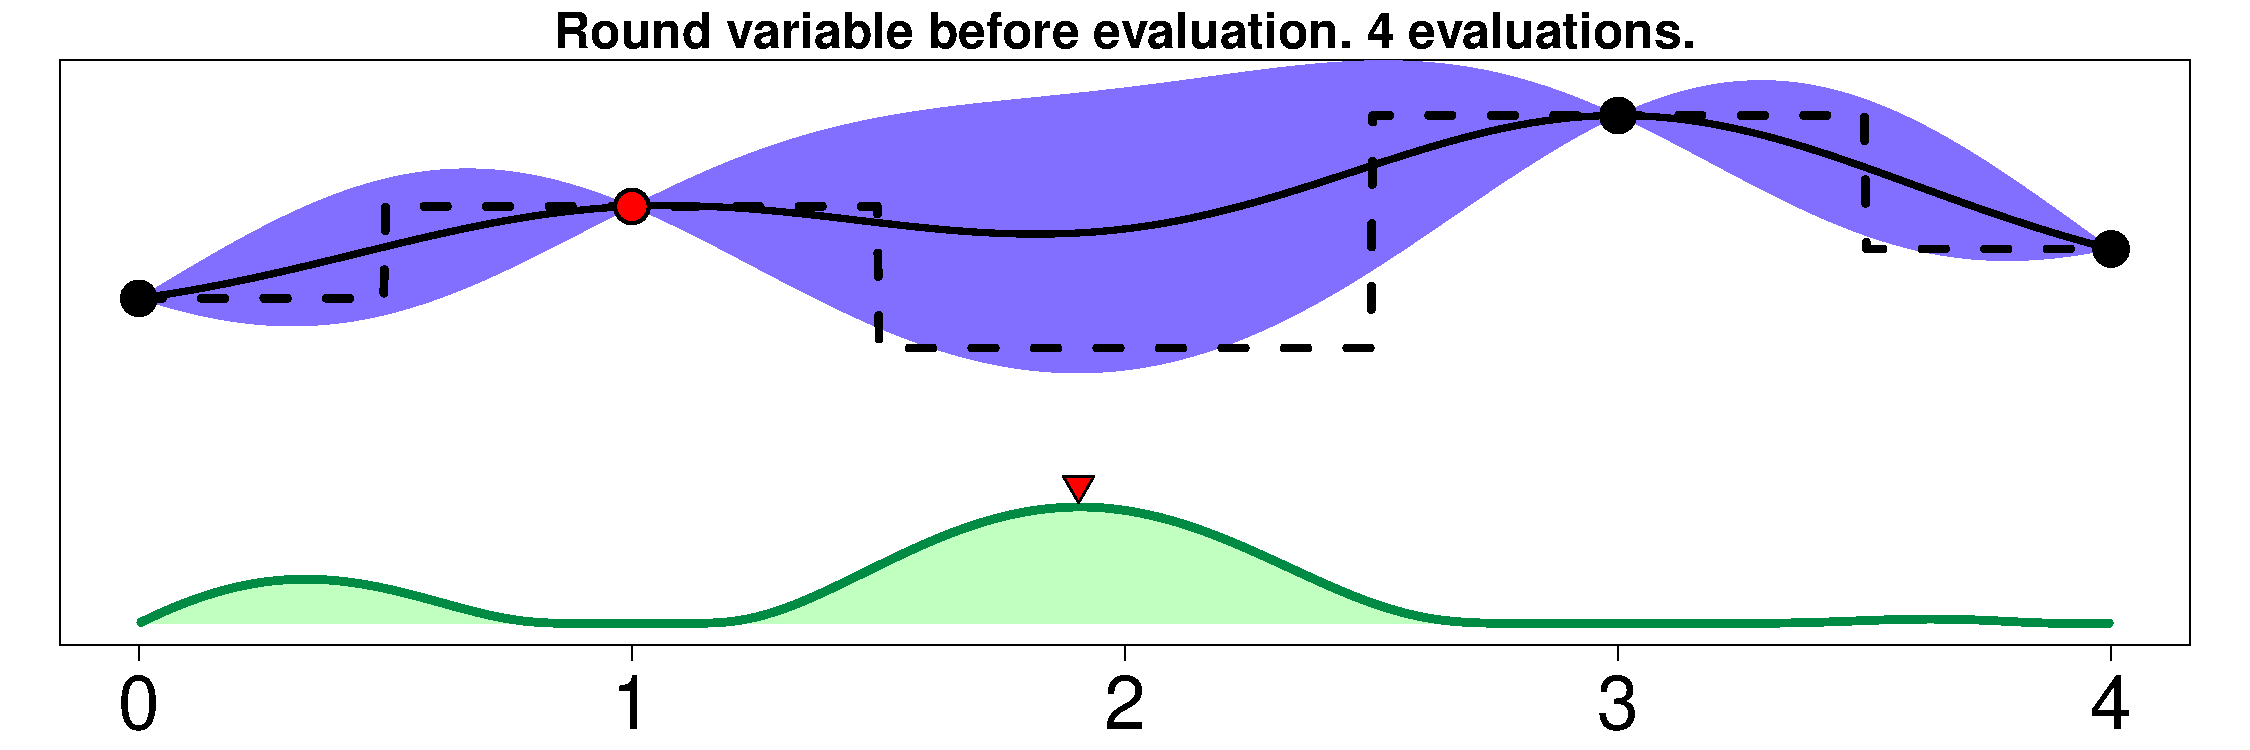
\includegraphics[width=0.45\linewidth]{Figures/integer/images/introduction/s4_before.pdf} &
        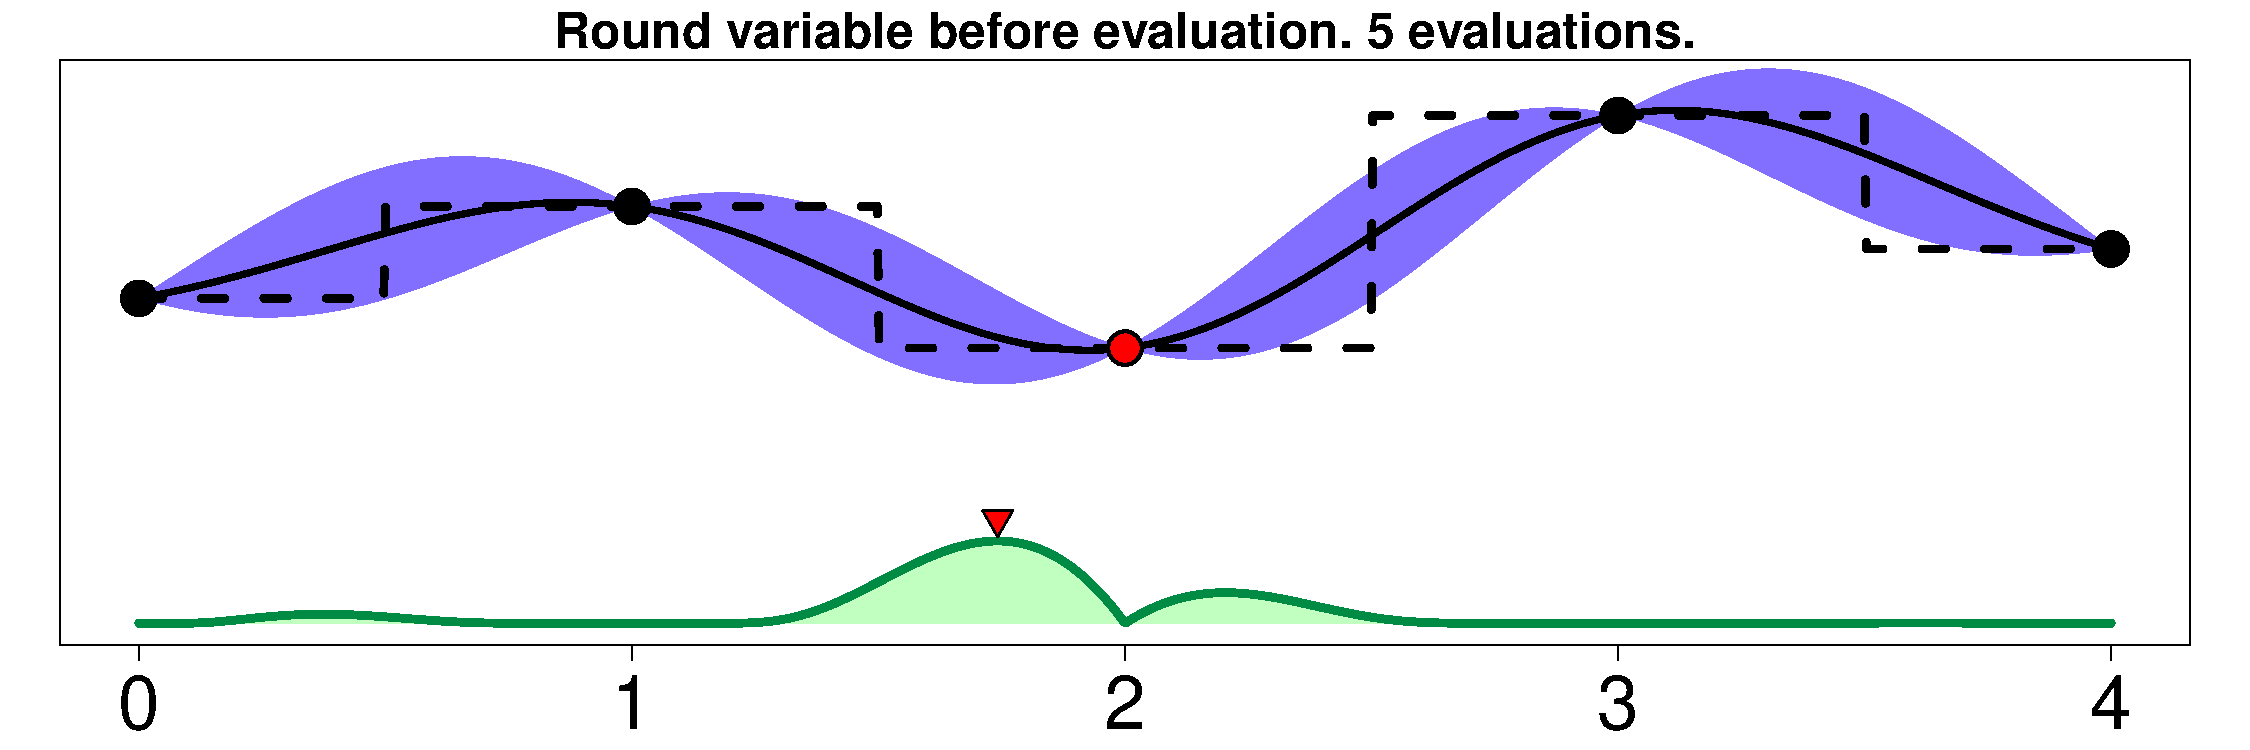
\includegraphics[width=0.45\linewidth]{Figures/integer/images/introduction/s5_before.pdf} \\
        \rotatebox{90}{\hspace{.7cm}{\bf \scriptsize Basic}} &
        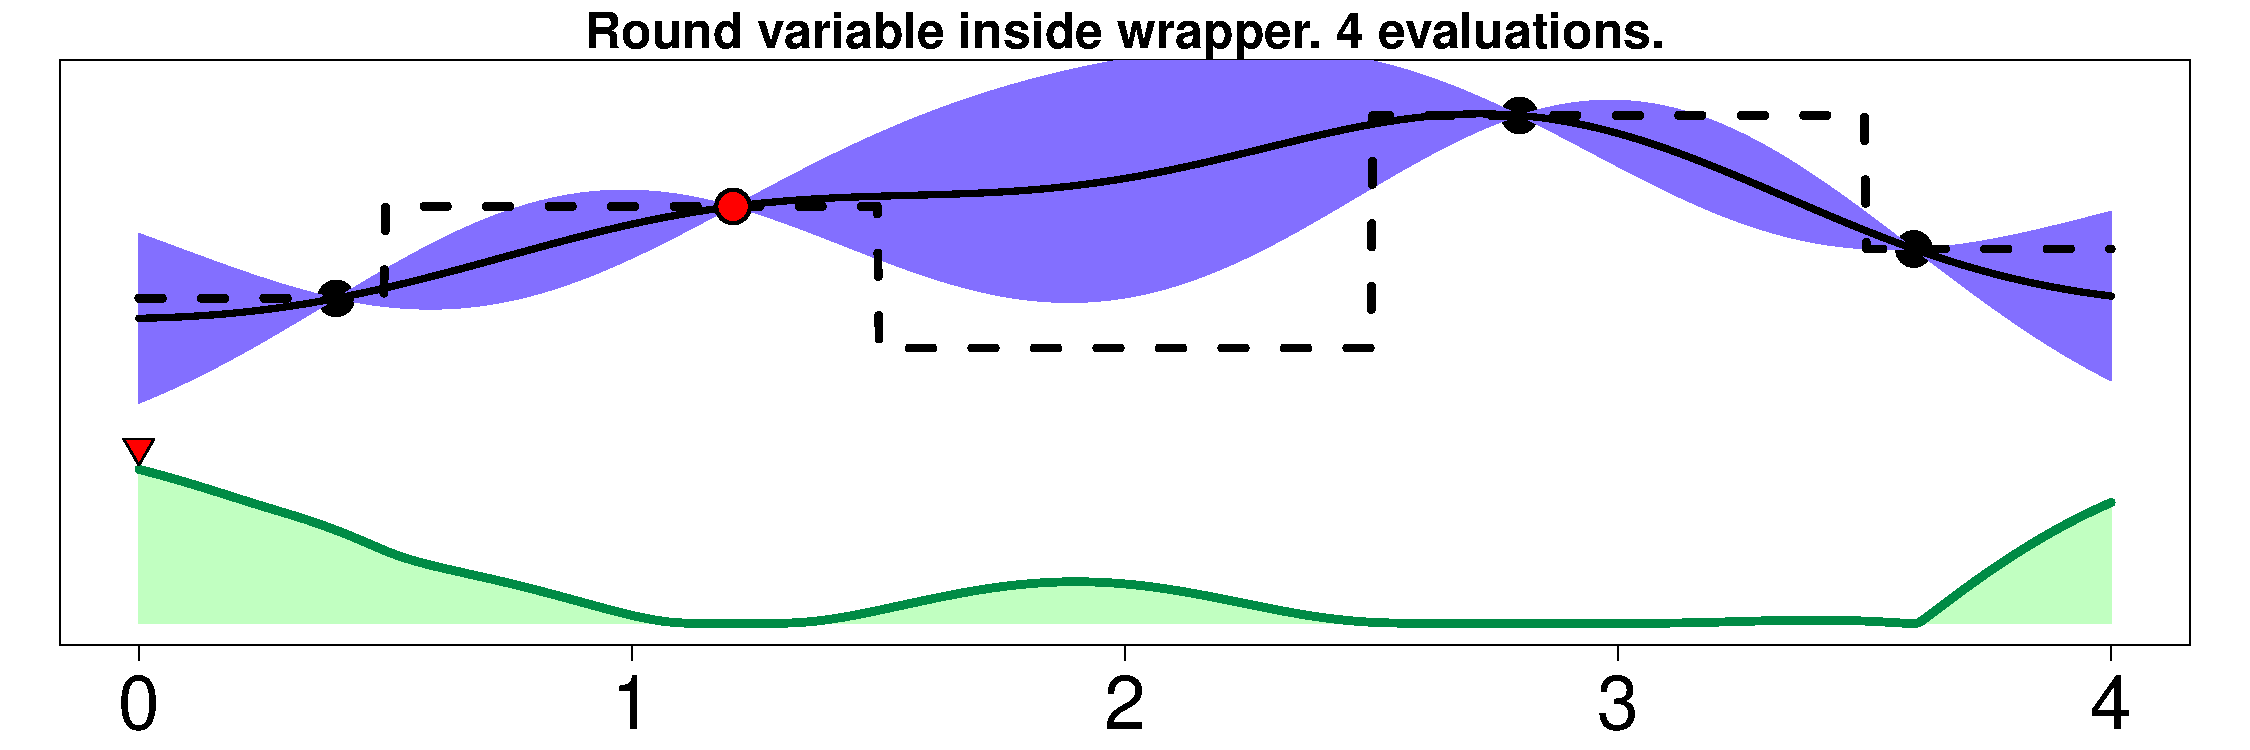
\includegraphics[width=0.45\linewidth]{Figures/integer/images/introduction/s4_inside.pdf} &
        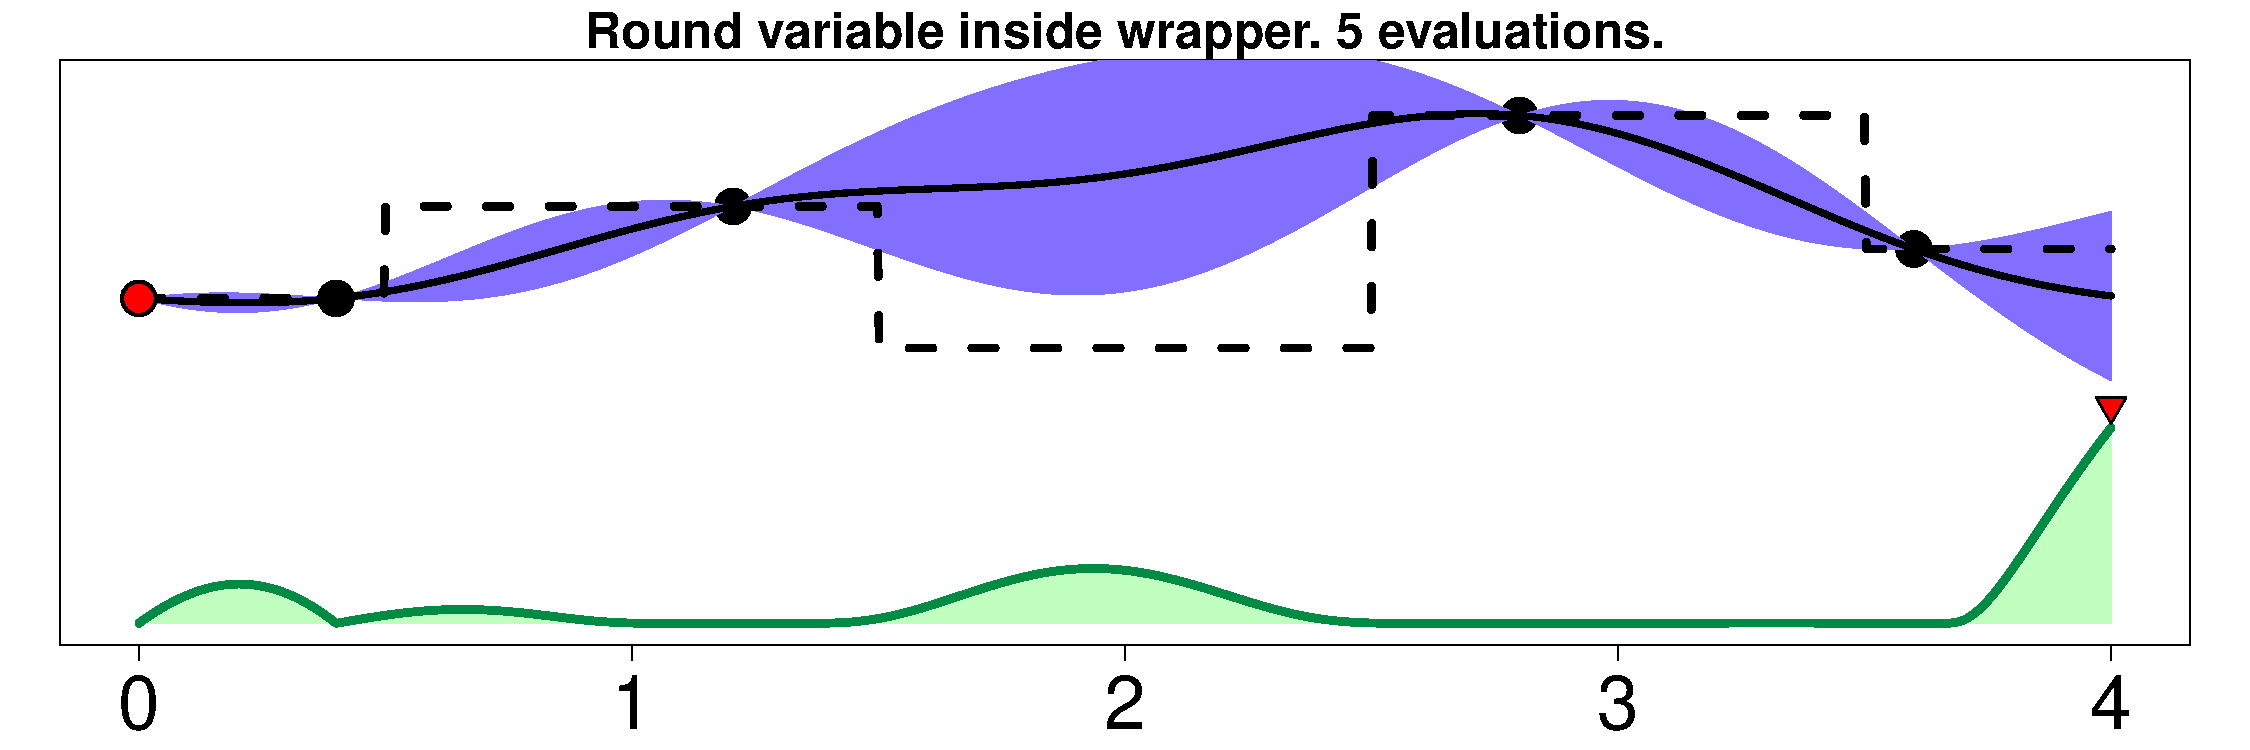
\includegraphics[width=0.45\linewidth]{Figures/integer/images/introduction/s5_inside.pdf} \\
        \rotatebox{90}{\hspace{.6cm}{\bf \scriptsize Proposed}} &
        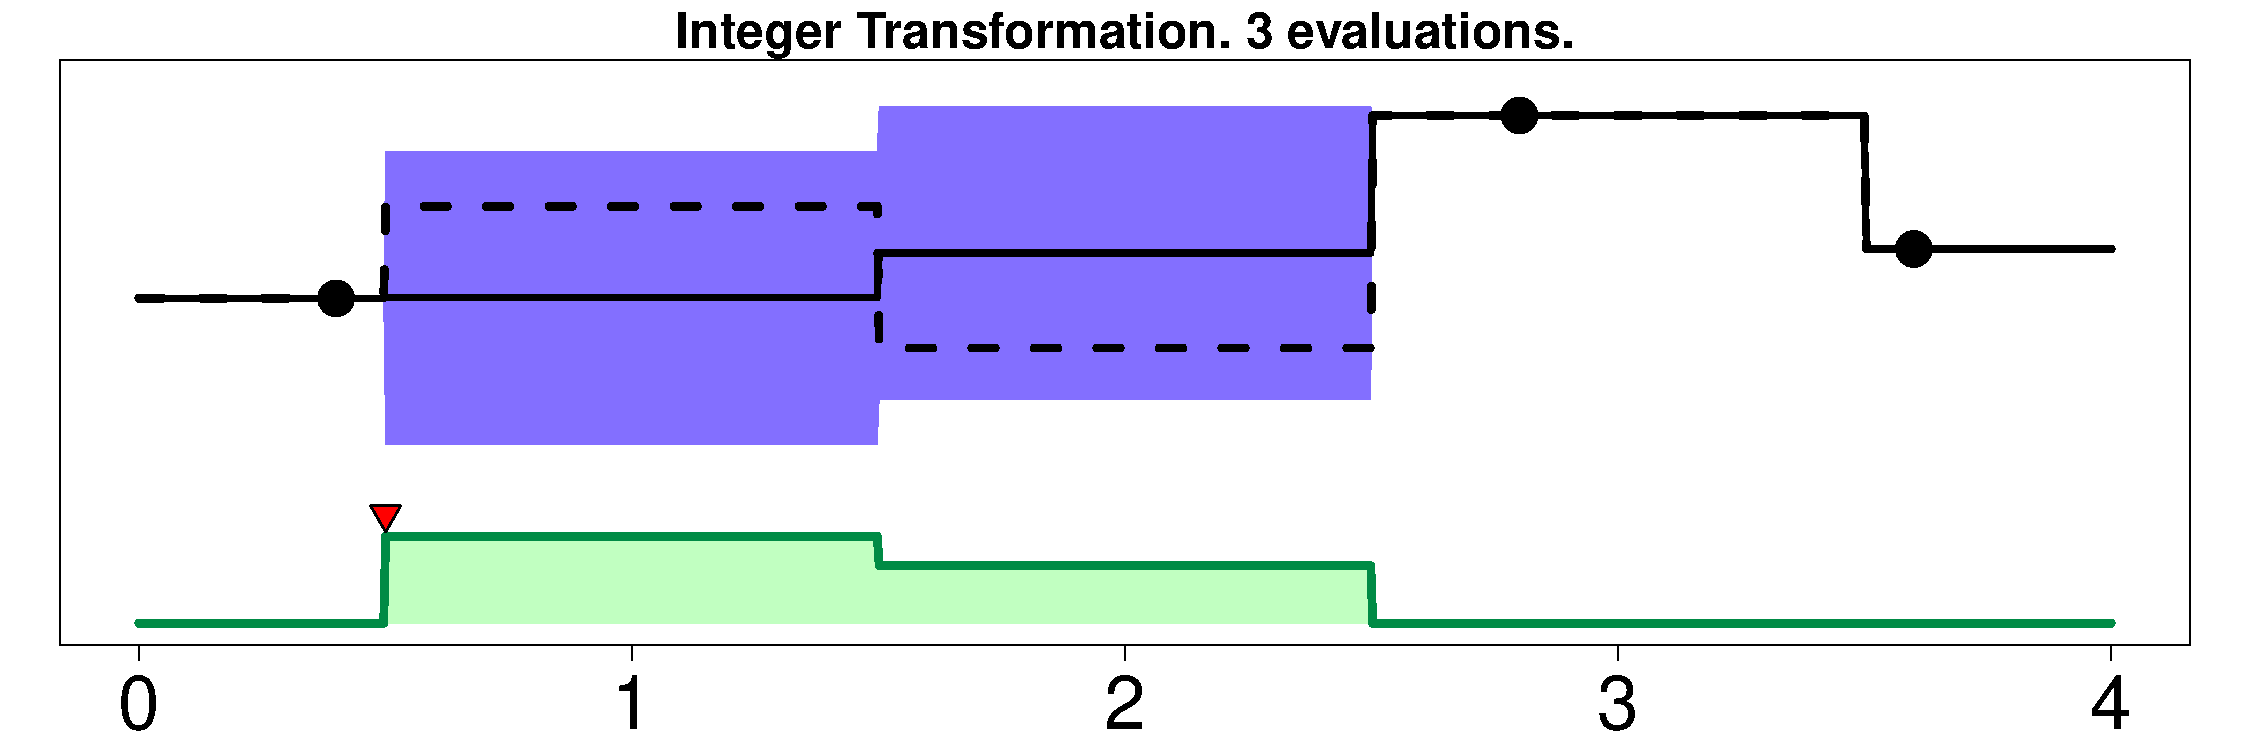
\includegraphics[width=0.45\linewidth]{Figures/integer/images/introduction/s3_transform.pdf} &
        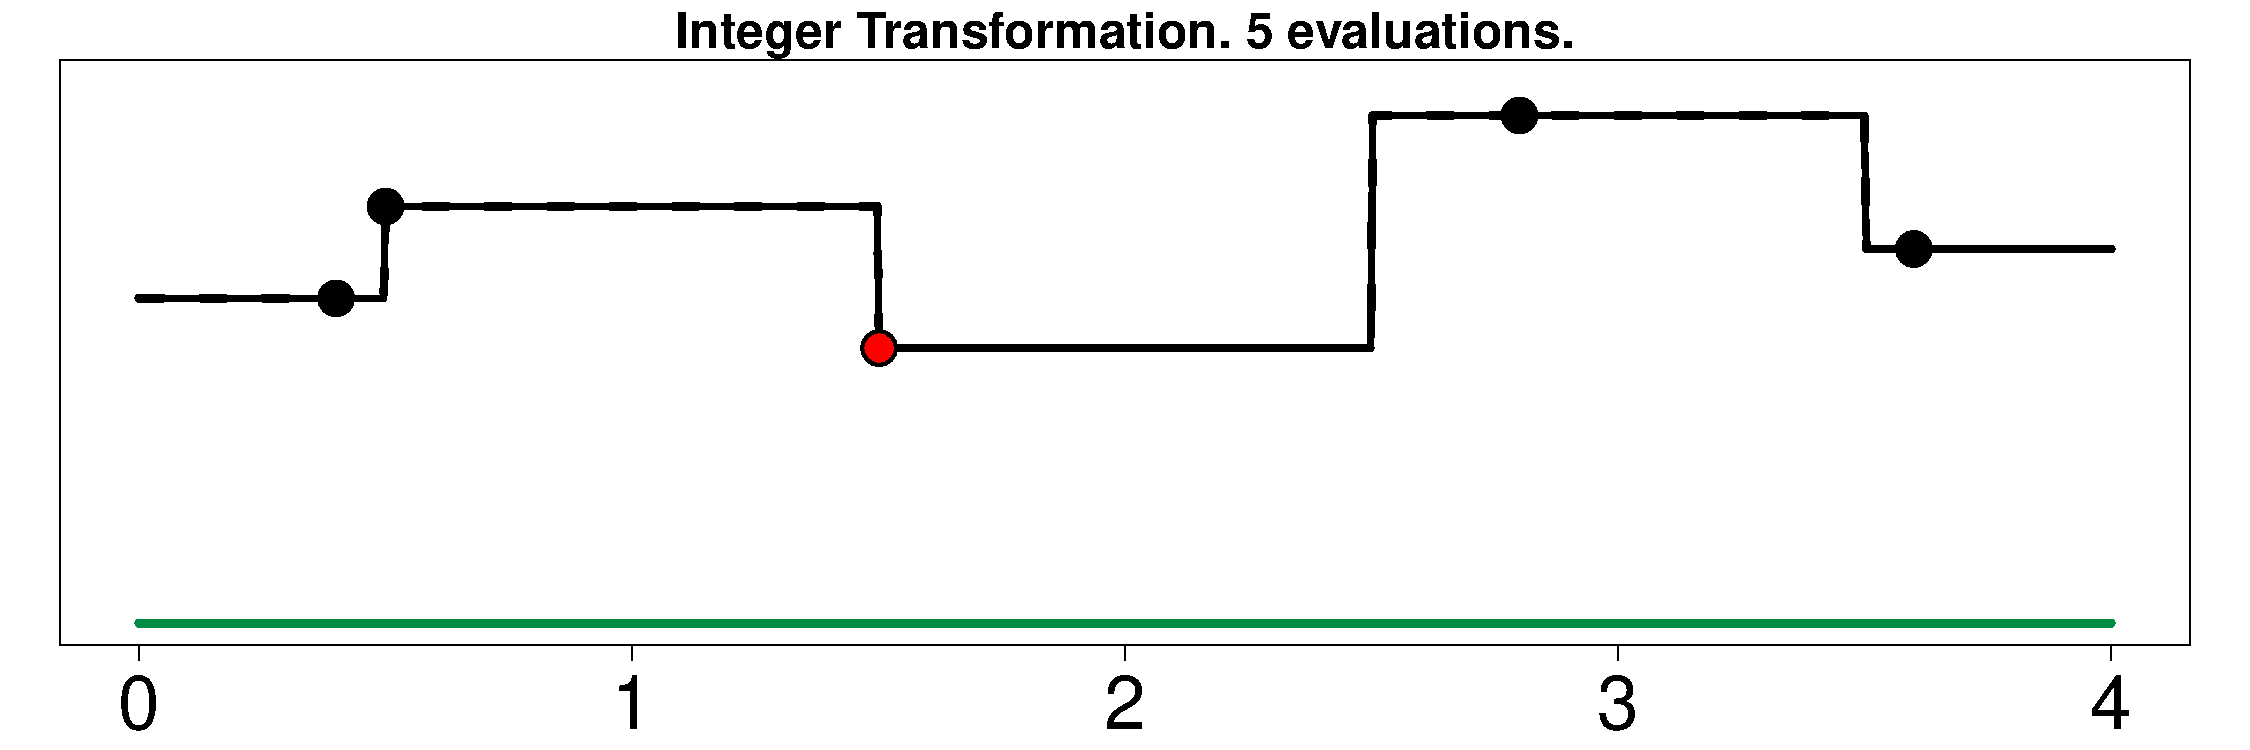
\includegraphics[width=0.45\linewidth]{Figures/integer/images/introduction/s5_transform.pdf} \\
\end{tabular}
\caption{{\small Different methods for dealing with integer-valued variables.
At the top of each image, we show a GP fit to the data (posterior mean and 1-std confidence interval, in purple)
that models a 1-dimensional objective taking values in the set $\{0,1,2,3,4\}$ (dashed line).
To display the objective we have rounded the real values at which to do the evaluation to the closest
integer. Below the GP fit, it is shown the acquisition function whose maximum is the recommendation for the next new
evaluation. Each column shows similar figures before and after evaluating a new point, respectively.
The proposed approach leads to no uncertainty about the objective after two evaluations.  Best seen in color.}}
\label{fig:methods}
\end{figure}

The previous problem can be easily solved. In the case of integer-valued variables, one can simply do
the rounding to the closest integer value inside the wrapper that evaluates the objective.
In the case of categorical variables, a similar approach can be followed inside the wrapper
using one-hot encoding. Namely, (i) look at which extra input variable has the largest
value, (ii) set that input variable equal to one, and (iii) set all other extra input variables equal to zero.
This basic approach is shown in the second row of Figure \ref{fig:methods} for the integer-valued case.
Here, the points at which the acquisition takes high values and the points at which the
objective is evaluated coincide. Thus, the BO method will tend to always perform evaluations at different input
locations, as expected. This will avoid the problem described before, in which the BO method may get stuck.
The problem is, however, that the actual objective is constant in the intervals that are rounded to
the same integer value. This constant behavior is ignored by the GP, which can lead to sub-optimal
optimization results. The same behavior is expected in the case of categorical input variables.

\subsection{Proposed Approach} \label{sec:integer}

We propose here a method to alleviate the problems of the basic approach described in Section \ref{sec:dealing}.
For this, we consider that the objective should be constant in those regions of the input space that
lead to the same input variable configuration on which the actual objective has to be evaluated.
This property can be easily introduced into the GP by modifying the covariance function
$k(\cdot,\cdot)$. Covariance functions are often stationary and only depend on the distance between the
input points \citep{rasmussen2003gaussian}. If the distance between two points is zero, the values of the function at
both points will be the same (the correlation is equal to one). Based on this fact, we suggest to transform
the input points to $k(\cdot,\cdot)$, obtaining an alternative covariance function $k'(\cdot,\cdot)$:
\begin{align}
k'(\mathbf{x}_i,\mathbf{x}_j) &= k(T(\mathbf{x}_i),T(\mathbf{x}_j)) \,,
\label{eq:covariance}
\end{align}
where $T(\mathbf{x})$ is a transformation in which all non real input variables of $f(\cdot)$ in $\mathbf{x}$
are modified as follows:
\begin{itemize}
\item The input variables corresponding to an integer-valued input variable are rounded to the closest integer value.
\item All extra input variables corresponding to the same categorical input variable are assigned zero value unless
        they take the largest value among the corresponding group of extra variables. If they take the largest value,
        they are assigned value one.
\end{itemize}
Essentially $T(\cdot)$ does the same transformation on $\mathbf{x}$ as the one described in Section
\ref{sec:basic_naive} for the basic approach inside the wrapper that evaluates the objective. Importantly, however,
this transformation takes place in the covariance function of the GPs, which will allow for a
better modeling of the objective.

The beneficial properties of $k'(\cdot,\cdot)$ when used for BO are illustrated in the
third row of Figure \ref{fig:methods} for the case of an integer-valued input variable.
We can see that the GP model correctly identifies that the objective function is constant
inside intervals of real values that are rounded to the same integer. The uncertainty is also
the same in those intervals, and this is reflected in the acquisition function. Furthermore, after performing
a single measurement in each interval, the uncertainty about $f(\cdot)$ goes to zero. This better modeling
of the objective is expected to be reflected in a better performance of the optimization process.
The same behavior is expected in the case of categorical variables.

In the case of integer-valued variables, the transformation $T(\mathbf{x})$ will round all integer-valued
variables values in $\mathds{R}$ to the closest integer $k \in \mathds{Z}$. The set of integer values,
$\mathds{Z}$, has a notion of order. That is, for all $z \in \mathbb{Z}$, we can define operators of order
that involve two values: $<,>,\leq$ and $\geq$, such that $z_i < z_j$, $z_j > z_i$, $z_i \leq z_j$ and
$z_j \geq z_i$, having that $z_i,z_j \in \mathbb{Z}$. This order will be preserved by the
resulting transformation. More precisely, assume an integer input variable and that $T(\mathbf{x})$ and $T(\mathbf{x}')$
only differ in the value of such integer input variable. The prior covariance between
$f(\mathbf{x})$ and $f(\mathbf{x}')$ under $k(T(\mathbf{x}),T(\mathbf{x}'))$ will be higher the closer the
corresponding integer values of $T(\mathbf{x})$ and $T(\mathbf{x}')$ are one from another. Therefore, the GP
will be able to exploit the smoothness in the objective $f(\cdot)$ when solving the optimization problem.

In the case of categorical variables (\emph{e.g.}, variables that can take values such as
\emph{red}, \emph{green}, \emph{blue}) there is no notion of order. That is, the operators
$<,>,\geq$ and $\leq$ have no meaning nor purpose. One cannot compare two different
values $c_1,c_2$ of any categorical-valued set $\mathds{C}$ according to these operators. However,
what does exist in a categorical set is a notion of equality or difference, given by the operators $=,\neq$.
The proposed transformation is able to preserve this notion of no order and notion of equal or
different. More precisely, assume a single categorical variable and that $T(\mathbf{x})$ and $T(\mathbf{x}')$
only differ in the values of the corresponding extra variables associated to that categorical variable.
The prior covariance between $f(\mathbf{x})$ and $f(\mathbf{x}')$ under
$k(T(\mathbf{x}),T(\mathbf{x}'))$ will be the same as long as $T(\mathbf{x})$ and $T(\mathbf{x}')$
encode a different value for the categorical variable. Of course if $T(\mathbf{x})$ and $T(\mathbf{x}')$
encode the same value for the categorical variable, the covariance will be maximum.

It is straight-forward to show that the proposed transformation generates a valid kernel function.
In particular, a kernel is valid if we can find an embedding $\phi(\cdot)$ such that $k(\mathbf{x},\mathbf{x}')=
\phi(\mathbf{x})^\text{T}\cdot \phi(\mathbf{x})$ \cite{shawe2004kernel}. Assume that the original kernel is valid
and hence $k(\mathbf{x},\mathbf{x}')= \phi(\mathbf{x})^\text{T}\cdot \phi(\mathbf{x})$ for some embedding $\phi(\cdot)$.
Then $k(T(\mathbf{x}),T(\mathbf{x}'))= \phi(T(\mathbf{x}))^\text{T}\cdot \phi(T(\mathbf{x}))$, and the  embedding
of the resulting kernel is simply given by $\phi(T(\cdot))$.

\subsubsection{Visualization of the Proposed Transformation} \label{sec:visual}

Figure \ref{fig:posterior} illustrates the modeling properties of the proposed transformation in the case of a real
and an integer-valued variable given by Equation (\ref{eq:covariance}). It shows the mean and standard deviation of the posterior
distribution of a GP given some observations. It compares results with a standard GP that does not use the proposed
transformation. In this case, the data has been sampled from a GP using the covariance function in Equation (\ref{eq:covariance})
with $k(\cdot,\cdot)$ the squared exponential covariance function \citep{rasmussen2003gaussian}. One dimension takes continuous
values and the other dimension takes values in $\{0,1,2,3,4\}$. Note that the posterior distribution captures the constant
behavior of the function in any interval of values that are rounded to the same integer, only for the integer
dimension (top). A standard GP (corresponding to the basic approach in Section \ref{sec:dealing}) cannot capture
this shape (bottom).

\begin{figure}[htb]
\begin{center}
\begin{tabular}{lcc}
        \rotatebox{90}{\hspace{.2cm}{\bf \scriptsize Proposed Approach}} &
        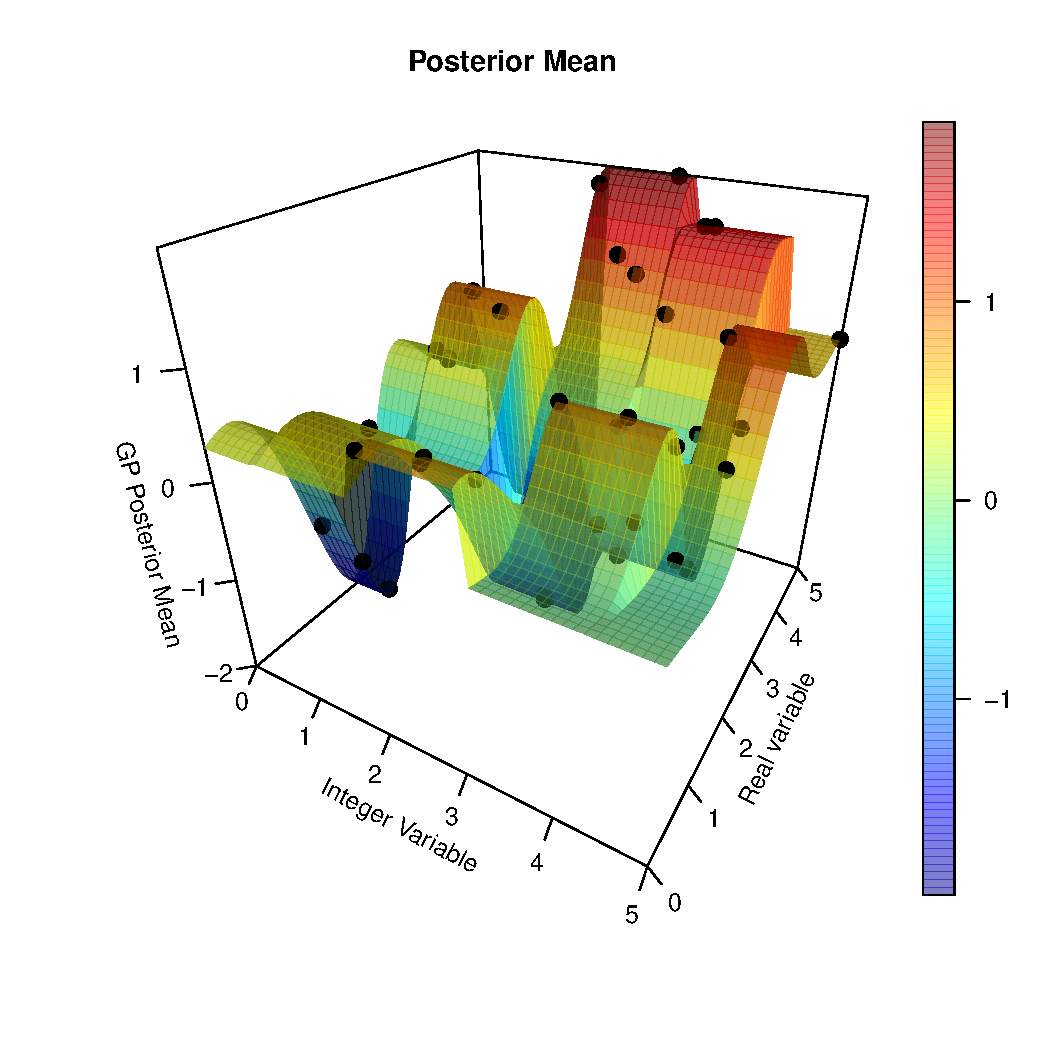
\includegraphics[width=0.375\linewidth]{Figures/integer/images/proposed_method/posterior_mean_persp3d_black.pdf} &
        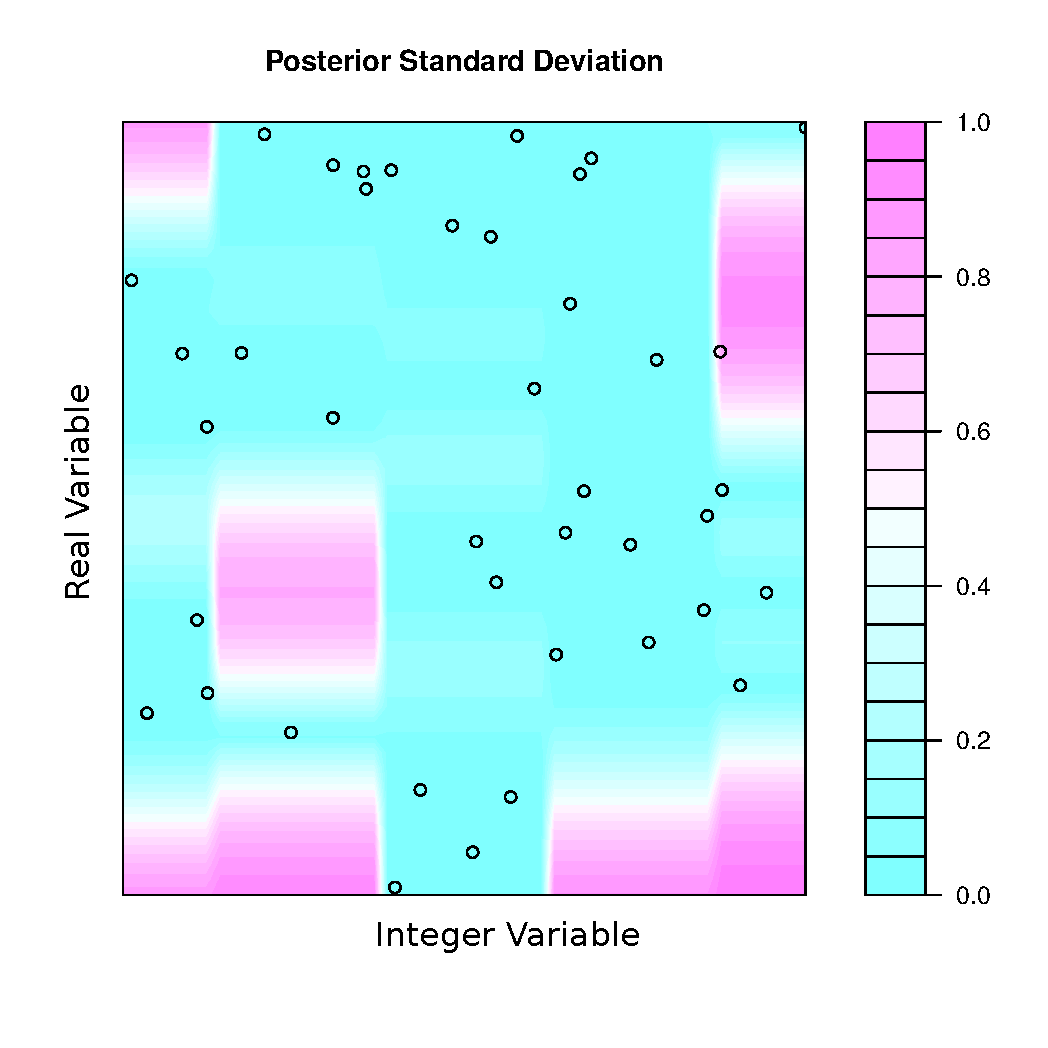
\includegraphics[width=0.375\linewidth]{Figures/integer/images/proposed_method/posterior_std_dev_contour.pdf} \\
        \rotatebox{90}{\hspace{.2cm}{\bf \scriptsize Standard GP}} &
        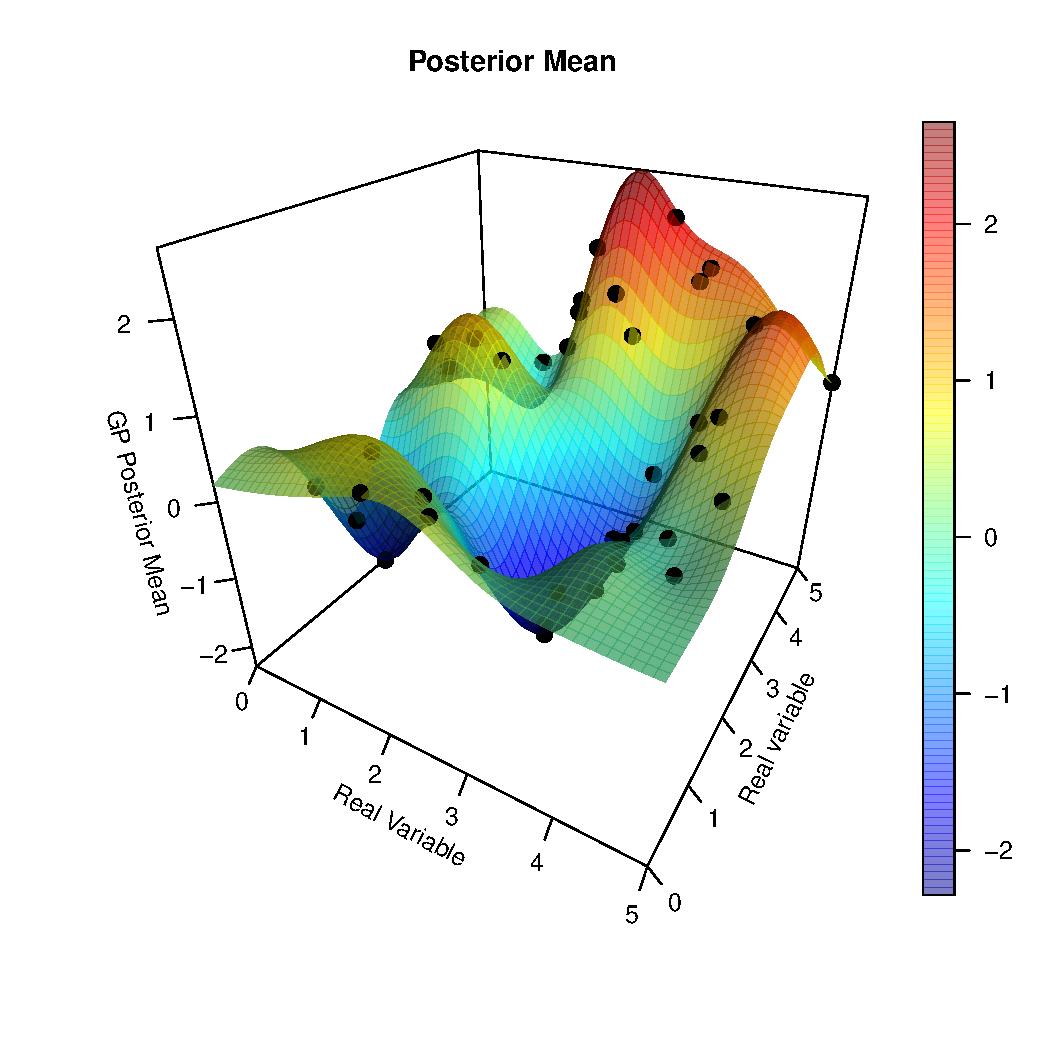
\includegraphics[width=0.375\linewidth]{Figures/integer/images/proposed_method/posterior_mean_persp3d_black_real.pdf} &
        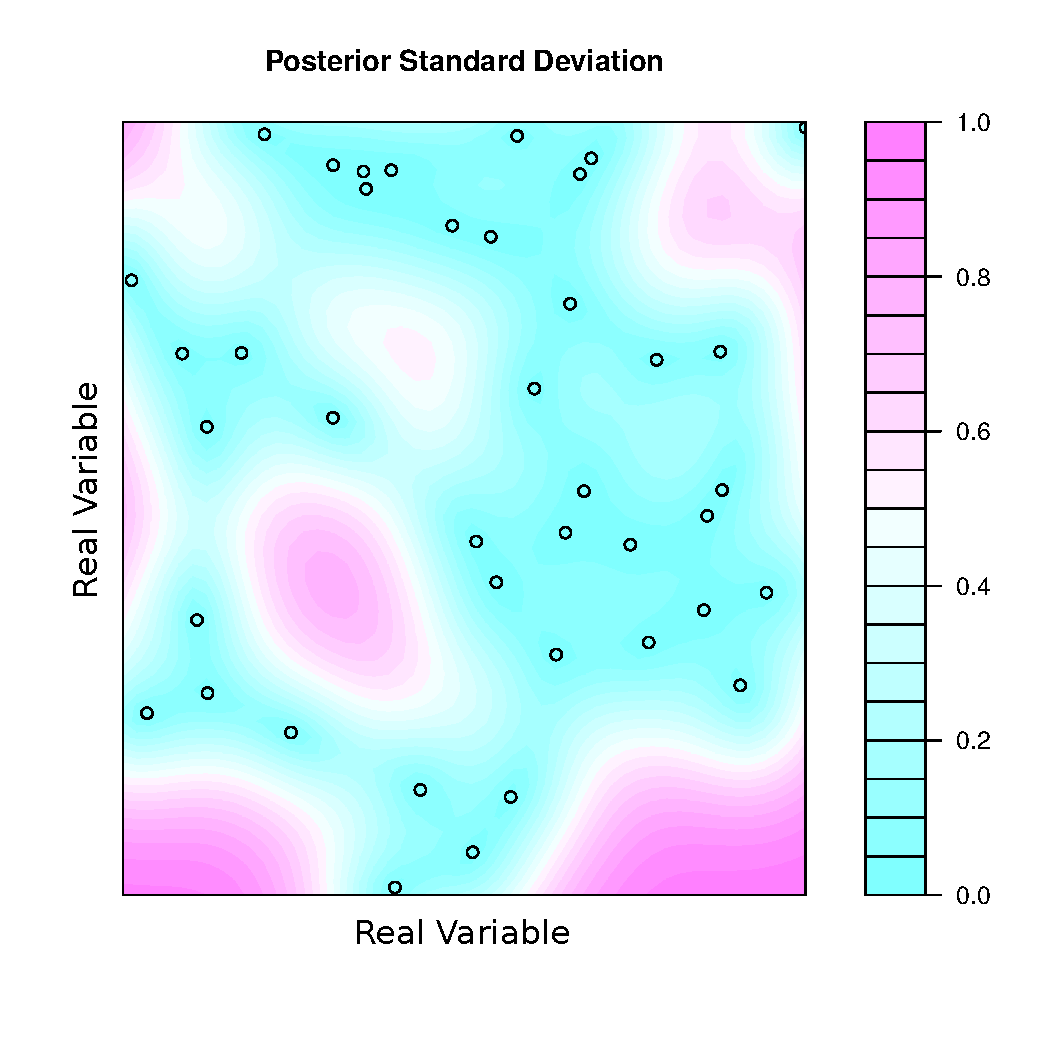
\includegraphics[width=0.375\linewidth]{Figures/integer/images/proposed_method/posterior_std_dev_contour_real.pdf} \\
\end{tabular}
\end{center}
\caption{{\small (top) Posterior mean and standard deviation of a GP model over a 2-dimensional space in which the first dimension
can only take $5$ different integer values and when the covariance function in Equation (\ref{eq:covariance}) is used. Note that the second
dimension can take any real value. (bottom) Same results for a GP model using a covariance function without the proposed
transformation.  Best seen in color.}}
\label{fig:posterior}
\end{figure}

Figure \ref{fig:posterior_categorical} illustrates the proposed transformation for the categorical case and a
single variable that can only take two values, \emph{e.g.}, \emph{True} and \emph{False}. Using one-hot encoding,
these two values will be represented as $(0,1)$ and $(1,0)$, respectively. In the naive approach described before, this
categorical variable will be replaced by two real variables taking values in the range $[0,1]$. Notwithstanding, any
combination of values in which the first component is larger than the second will lead to the configuration value $(1,0)$.
Conversely, any combination of values in which the second component is larger will lead to the configuration value $(0,1)$.
Therefore, the corresponding objective will be constant in those regions of the input space that lead to the same configuration.

\begin{figure}[htb]
\begin{center}
\begin{tabular}{lcc}
        \rotatebox{90}{\hspace{.2cm}{\bf \scriptsize Proposed Approach}} &
        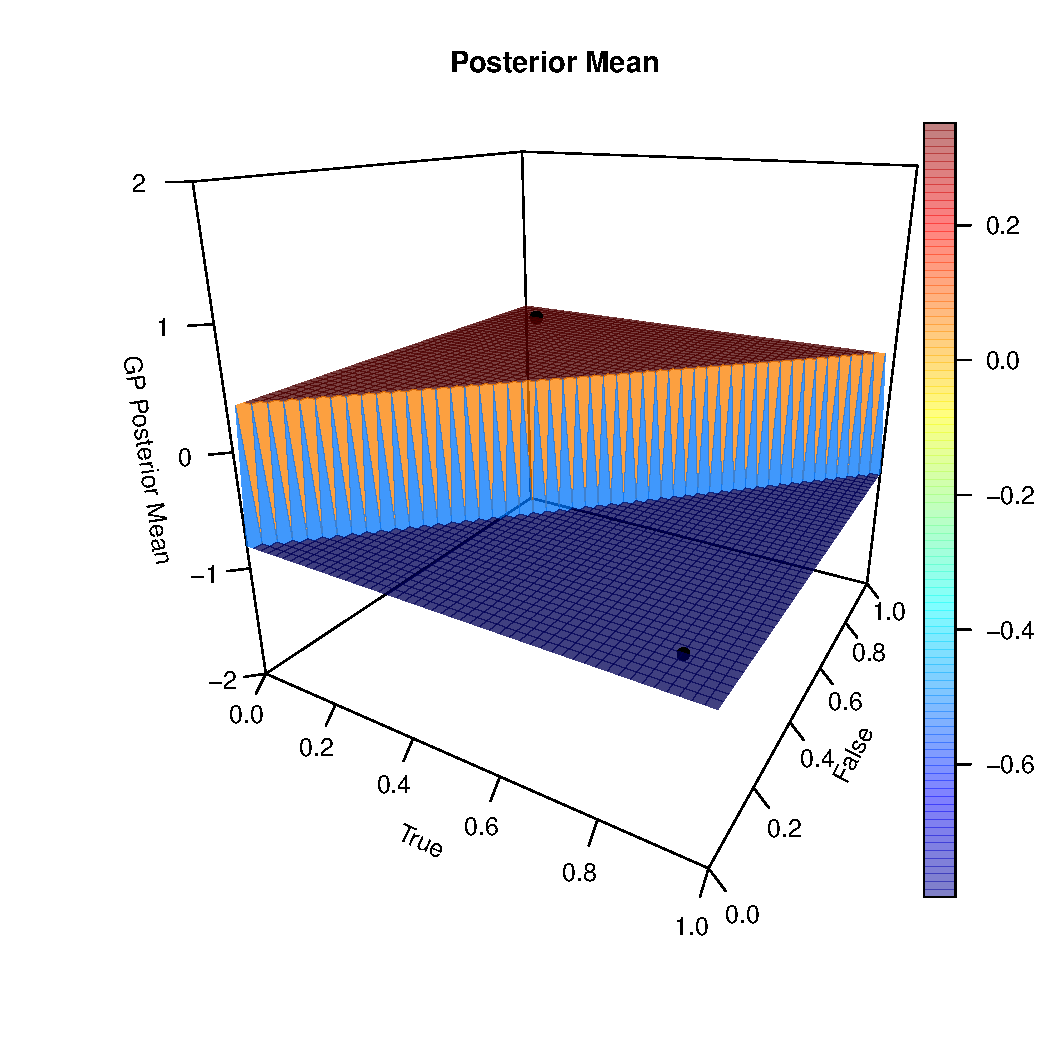
\includegraphics[width=0.35\linewidth]{Figures/integer/categorical/posterior_mean_perspective_categorical.pdf} &
        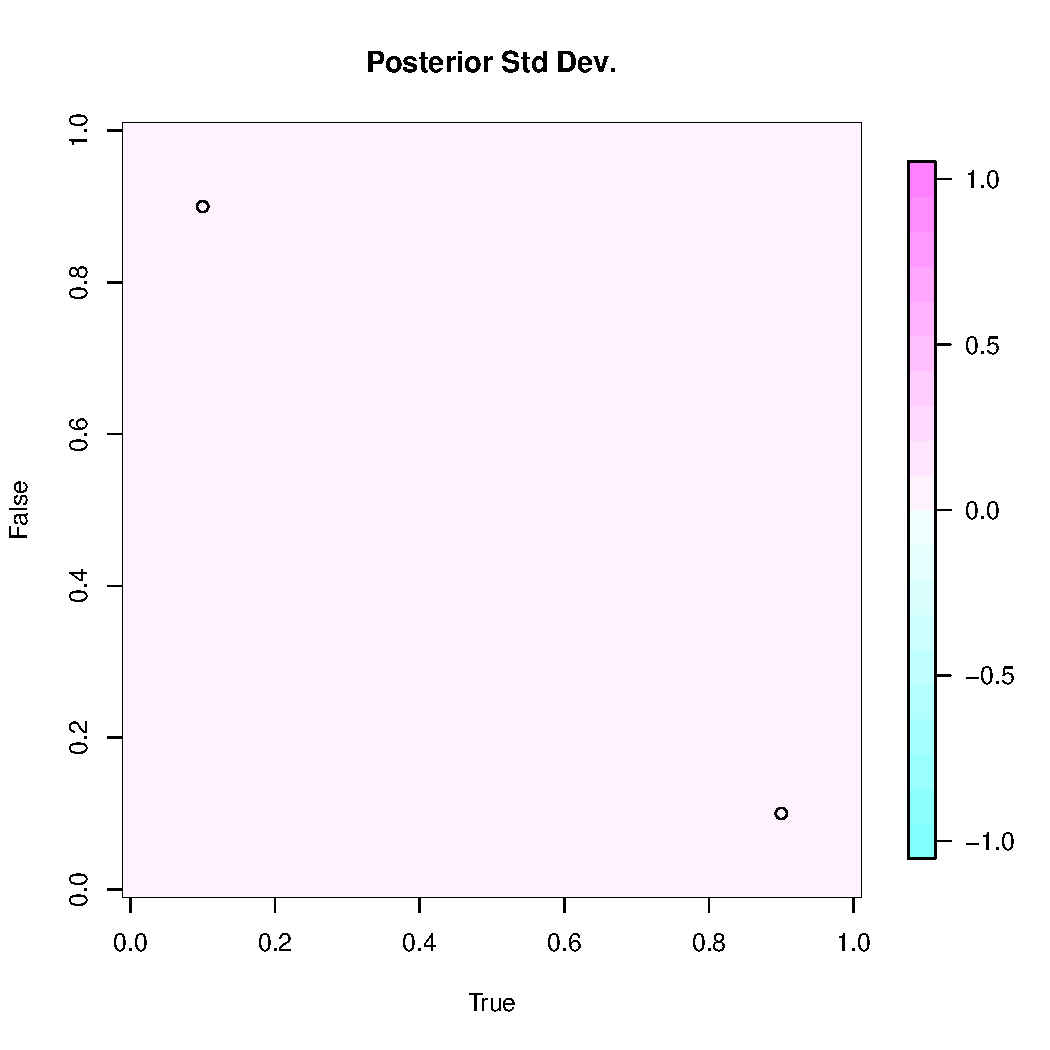
\includegraphics[width=0.35\linewidth]{Figures/integer/categorical/posterior_std_dev_contour_categorical.pdf} \\
        \rotatebox{90}{\hspace{.2cm}{\bf \scriptsize Standard GP}} &
        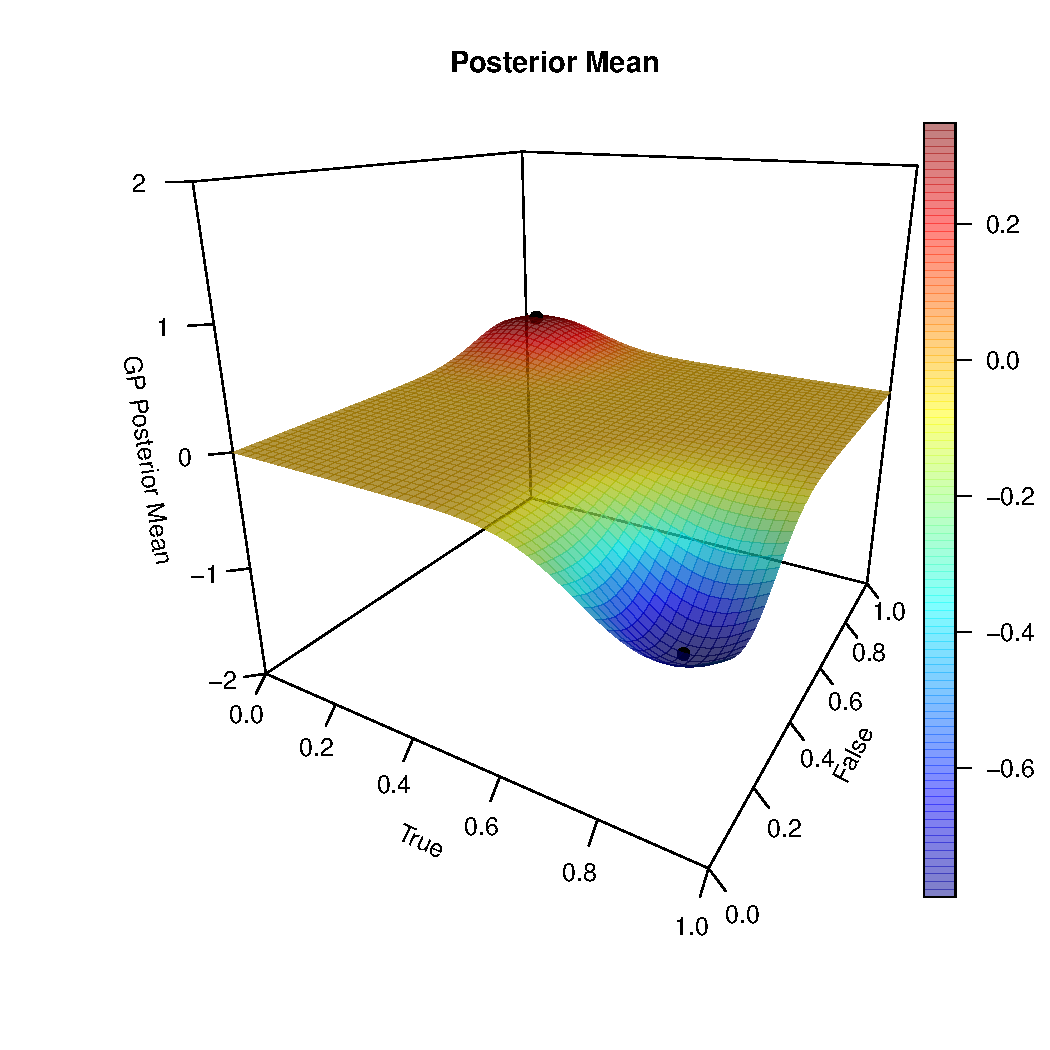
\includegraphics[width=0.35\linewidth]{Figures/integer/categorical/posterior_mean_perspective_real.pdf} &
        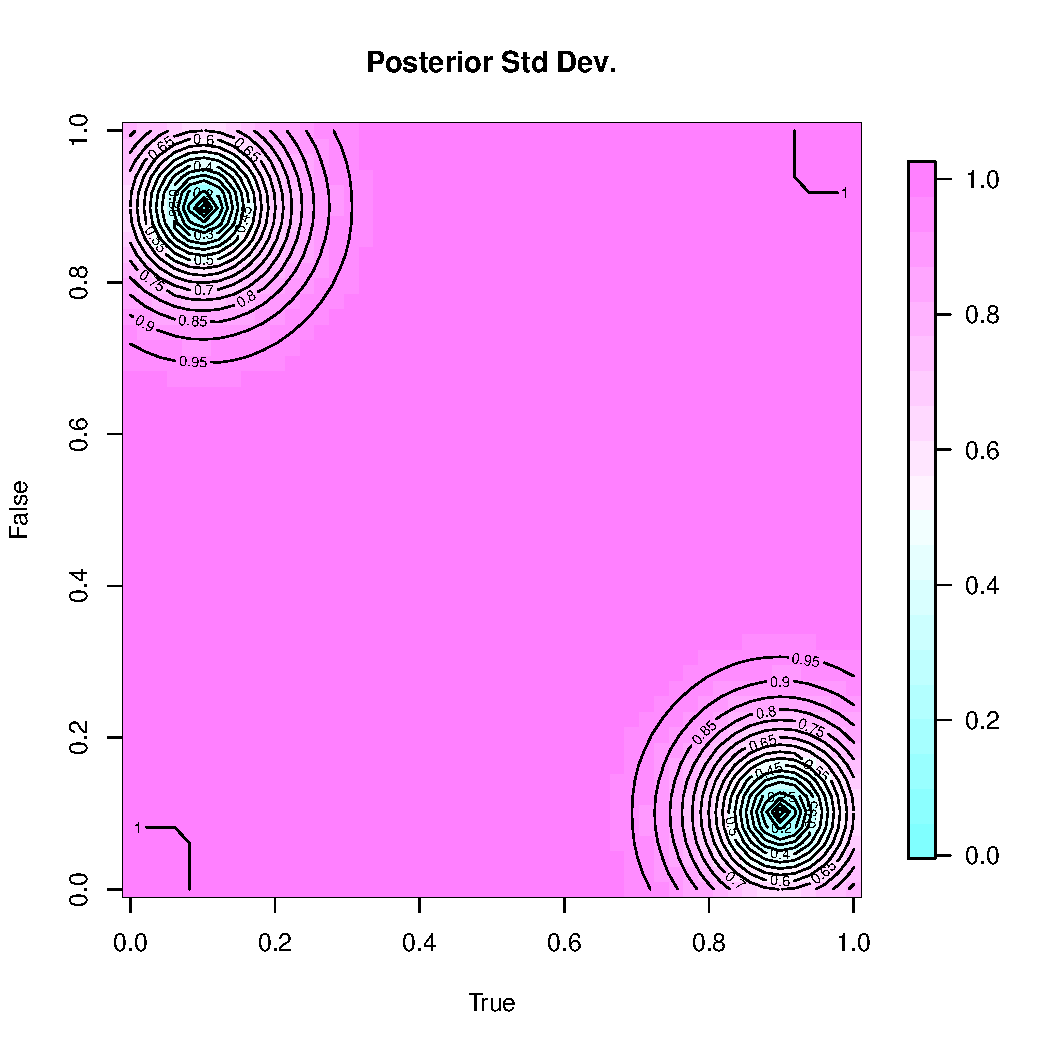
\includegraphics[width=0.35\linewidth]{Figures/integer/categorical/posterior_std_dev_contour_real.pdf} \\
\end{tabular}
\end{center}
\caption{{\small (top) Posterior mean and standard deviation of a GP model over a 1-dimensional binary variable.
The covariance function in Equation (\ref{eq:covariance}) is used. Same results for a GP model using a covariance function without the proposed
transformation.  Best seen in color.}}
\label{fig:posterior_categorical}
\end{figure}

This behavior is illustrated by Figure \ref{fig:posterior_categorical} (top), in which the posterior distribution of the GP is plotted
given two observations. In this case we use the proposed transformation of the covariance function.
Note that the uncertainty goes to zero after just having a single observation corresponding to
the \emph{True} value and a single observation corresponding to the \emph{False} value. This makes sense, because
the objective is constant in all those regions of the input space that lead to the same configuration of
the extra variables introduced in the input space. In Figure \ref{fig:posterior_categorical} (bottom) we show
that a standard GP cannot model this behavior, and the posterior distribution of the mean is not constant in
those regions of the input space that lead to the same configuration for the categorical variable.
Furthermore, the posterior standard deviation is significantly different from zero, unlike in the proposed approach.
Summing up, Figure \ref{fig:posterior_categorical} shows that by using the proposed covariance function, we are
better modeling the objective function, which in the end will be translated in better optimization results.

\subsection{Optimization of the Acquisition Function} \label{sec:acquisition}

A consequence of the transformation described in the previous section is that the
acquisition function will be flat in some regions of the input space, depending on the number of
integer and categorical variables. This behavior is illustrated in Figure \ref{fig:methods} for one
integer-valued variable. Often, the typical approach to optimize the acquisition is to evaluate it
first on a grid of points to search for a good candidate point at which to start a gradient-based search
using, \emph{e.g.}, L-BFGS. This is the approach employed by the BO software Spearmint. However, if the
acquisition function is not smooth, this may be sub-optimal. Assume that we want to optimize a function
with $D$ binary categorical inputs, with large $D$, for example, $30$. The best point after evaluating the
acquisition function on a grid is extremely unlikely to be the best among the $2^D$ choices, and the
gradient-based optimization of the acquisition function will not leave the starting point, since the
acquisition function is expected to be flat at the starting point.

To overcome this problem, we consider a block coordinate ascent optimization methodology which
iterates between optimizing the non-real variables (integer-valued and categorical) and real variables,
similar to the one-exchange neighborhood (OEN) strategy described in \citep{hutter2009automated,levesque2017bayesian}.
Our methodology consists in using the grid and the L-BFGS methods to optimize all real
variables and then, the OEN strategy to optimize the transformed integer and categorical variables.
The OEN strategy is a greedy method. Under it, one iteratively evaluates for each non-real dimension,
the corresponding neighbors of that dimension, and if some improvement is made in terms of the acquisition function, that new value is kept as the best
one. This process is repeated until no further progress is made. Of course, to evaluate the quality of each neighbor,
for a given integer-valued or categorical dimension, the real variables have to be optimized. For that task, we use the
L-BFGS method.

Of course, at this point one may ask whether the proposed transformation of the GP covariance function is beneficial
at all, and if simply optimizing the acquisition function as described here could be enough. To answer this question,
we have also implemented block coordinate ascent optimization methodology without transforming the integer-valued
and categorical variables in the GP covariance function. We compared in a toy problem the results given by both approaches,
the proposed approach and the alternating optimization methodology alone, which we refer to as OEN optimization only.

Figure \ref{fig:comparison} shows the evaluations performed by the proposed approach and by OEN optimization only
in a 2-dimensional optimization problem with one real variable and one integer-valued variable taking 5 different values.
The contour curves show the value of the acquisition function. We show results after 10, 20 and 30 evaluations.
We observe that the proposed approach performs a more evenly evaluation of the input space. By contrast, the OEN
optimization only strategy, which does not make use of the proposed transformation, tends to concentrate all
evaluations in a particular region of the input space. This is a consequence of using a model (\emph{i.e.}, a GP
without the proposed transformation) that ignores that the actual objective will take the same value in those regions
of the input space that lead to the same integer value. In any case, our experiments  show that OEN optimization 
only often performs better than the basic approach described in Section \ref{sec:dealing},
which simply uses a grid of points combined with L-BFGS to optimize the acquisition function with respect to all input variables,
independently of whether they take real, integer or categorical values.

\begin{figure}[htb]
\begin{center}
\begin{tabular}{lccc}
        & {\bf 10 evaluations} & {\bf 20 evaluations} & {\bf 30 evaluations} \\
        \rotatebox{90}{\hspace{0.5cm}{\bf \scriptsize OEN Opt. Only}} &
        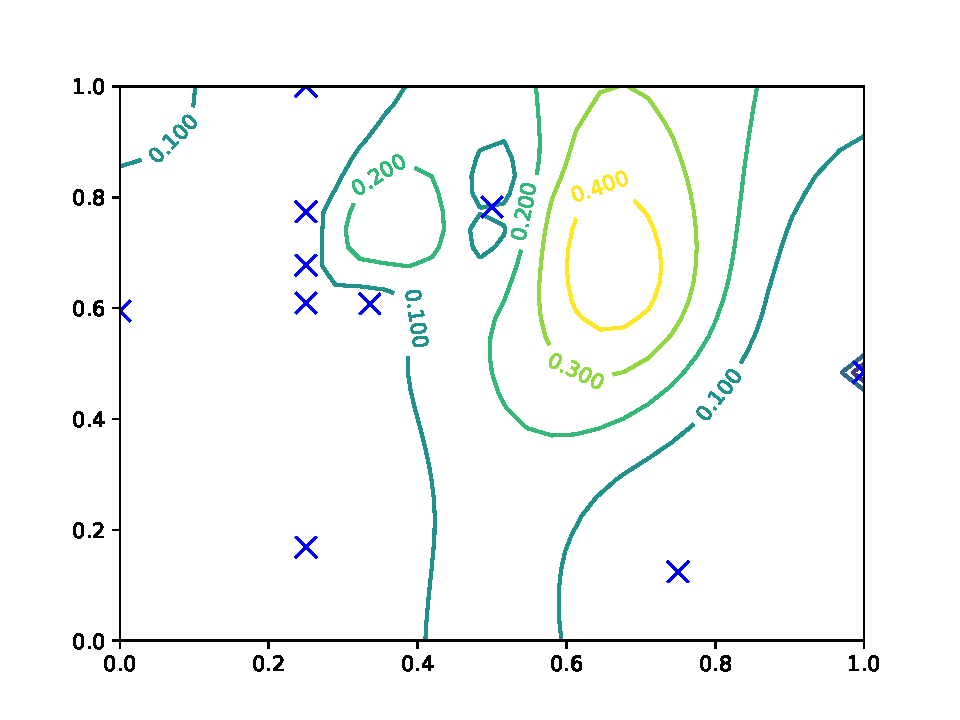
\includegraphics[width=0.3\linewidth]{Figures/integer/toy/oen_1.pdf} &
        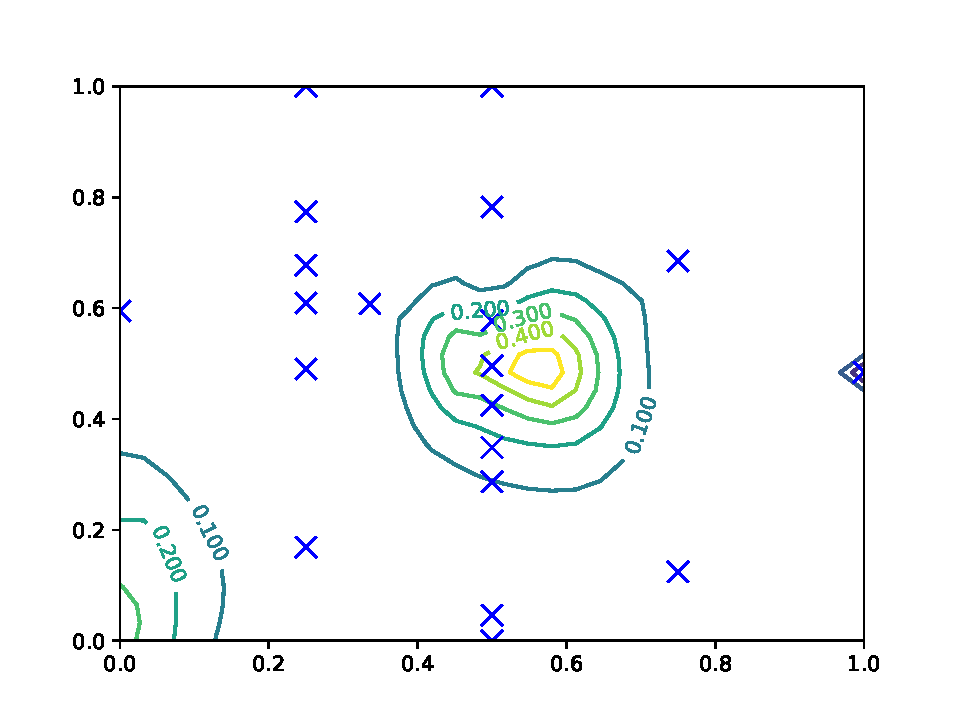
\includegraphics[width=0.3\linewidth]{Figures/integer/toy/oen_2.pdf} &
        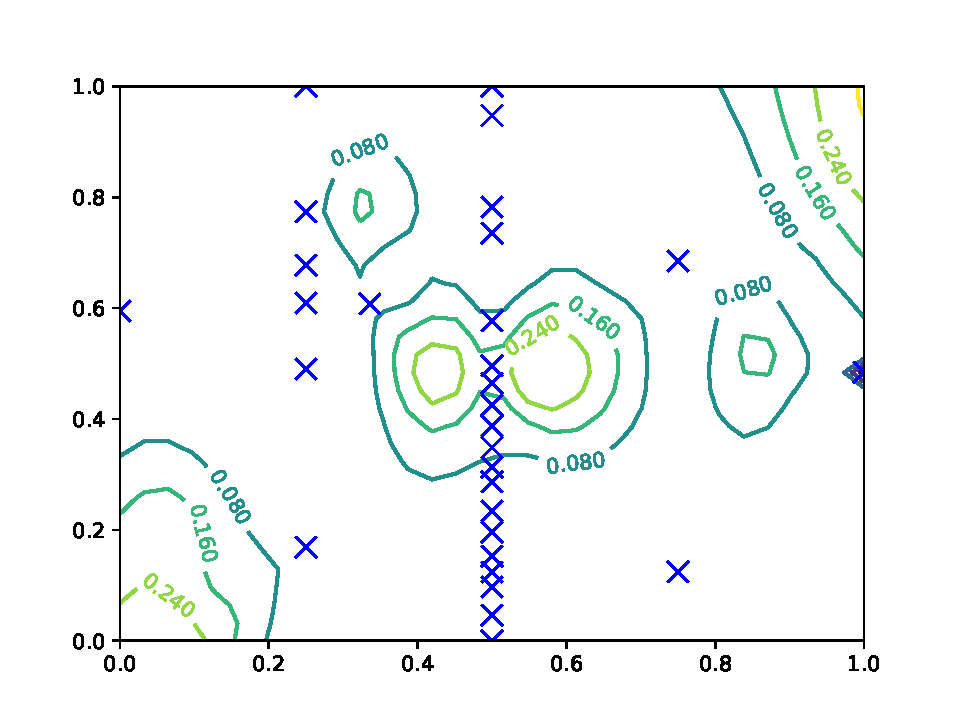
\includegraphics[width=0.3\linewidth]{Figures/integer/toy/oen_3.pdf} \\
        \rotatebox{90}{\hspace{.1cm}{\bf \scriptsize Proposed Approach}} &
        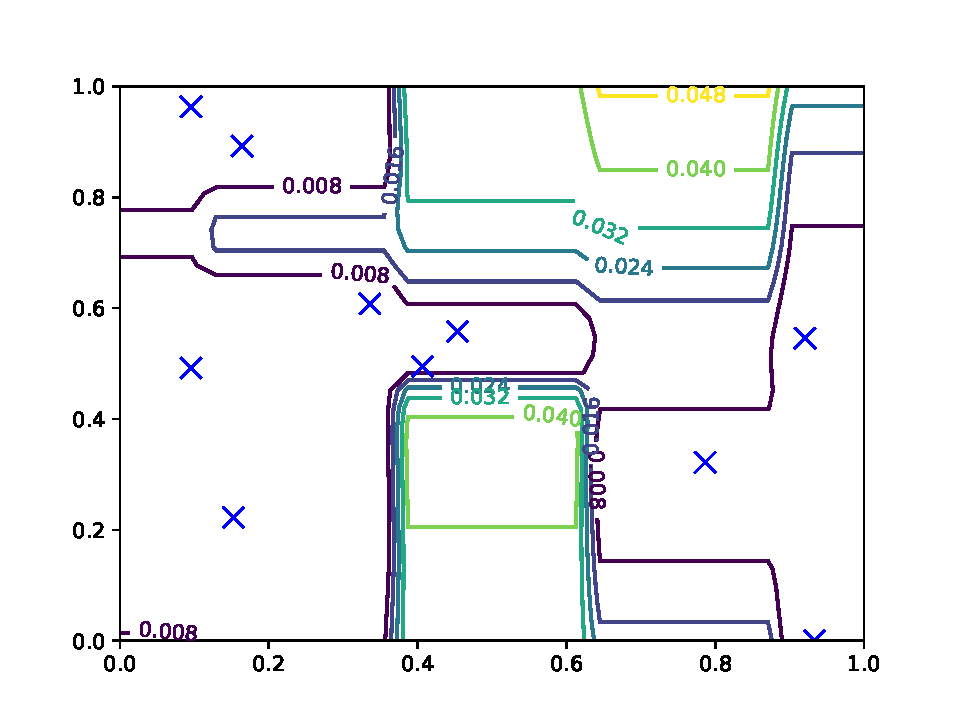
\includegraphics[width=0.3\linewidth]{Figures/integer/toy/proposed_1.pdf} &
        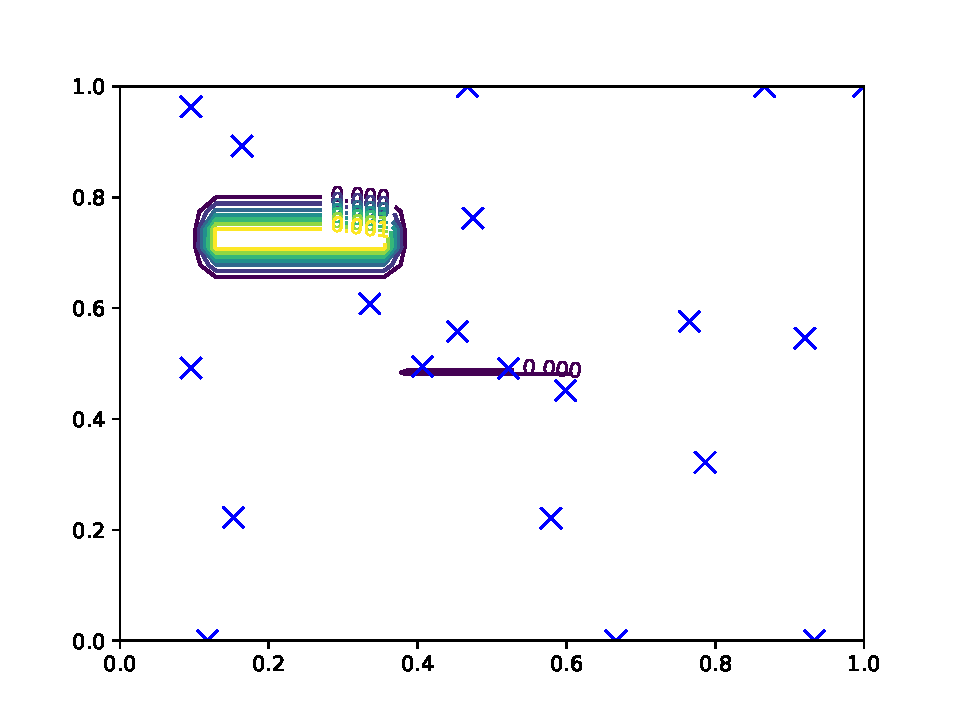
\includegraphics[width=0.3\linewidth]{Figures/integer/toy/proposed_2.pdf} &
        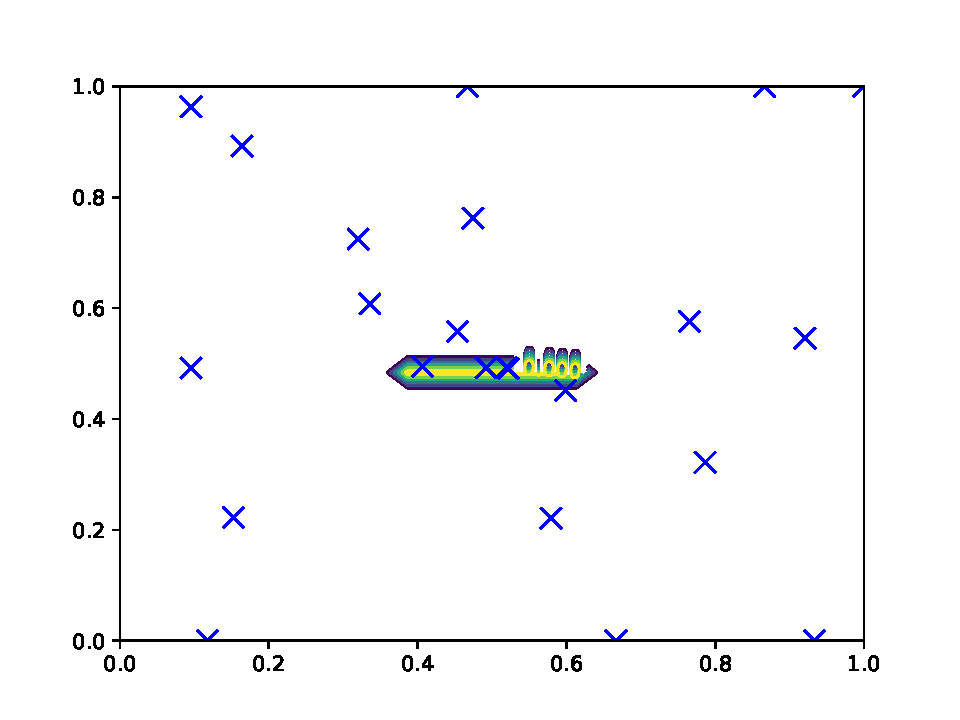
\includegraphics[width=0.3\linewidth]{Figures/integer/toy/proposed_3.pdf} \\
\end{tabular}
\end{center}
\caption{{\small Evaluations plotted by crosses performed by the OEN optimization only
method (top) and the proposed approach (bottom) of a 2-dimensional sample from a GP where
one of the variables is integer-valued with range $5$. The contour represents the value of the
acquisition function in the input space. From left to right, acquisition function with 10, 20 and
30 evaluations. Best seen in color.}}
\label{fig:comparison}
\end{figure}


\subsection{Dealing with Combinatorial-Valued Variables}
In addition to the proposed transformation, we extended this method to cover combinatorial-valued variables. We define a combinatorial-valued variable as a variable whose values are the power set of the values of a categorical variable. We can represent by using the categorical transformation a combinatorial-valued variable as a binary set of categorical variables. Each value of the combinatorial-valued variable is modelled by a binary categorical-valued variable. If the combinatorial-valued variable is the power set of a $D$-dimensional categorical-valued variable, the GP will require $2D$ dimensions to model a combinatorial-valued variable by using this approach.
Full representation of a combinatorial-valued variable as a categorical-valued variable which values are the power set of the values of the categorical variable. If the combinatorial-valued variable is the power set of a $D$-dimensional categorical-valued variable, the GP will require $2^D$ dimensions to model a combinatorial-valued variable by using this approach.

\section{Related Work}

We describe here two approaches that can be used as an
alternative to BO methods using GPs when categorical and/or
integer-valued variables are present in a black-box optimization problem. These
are Sequential model-based optimization for general algorithm configuration (SMAC) and the Tree-structured Parzen Estimator Approach (TPE)
\citep{hutter2011sequential} \citep{bergstra2011algorithms}. Both can naturally handle integer and categorical-valued
variables. SMAC is present in the popular machine learning tool AutoWeka \citep{thornton2013auto}.
TPE is used in the HyperOpt tool \citep{bergstra2013hyperopt}.

SMAC uses a random forest as the underlying surrogate model of the black-box
objective \citep{breiman2001random}. The predictive distribution given by
this model is used to select promising parameter values on which the objective should
be evaluated. In random forest $T$ random regression trees are iteratively fit using
each time a bootstrap sample of training data. Each bootstrap sample is obtained by drawing
with replacement from the observed data $N$ instances. Furthermore, in random forest, at each node,
a randomly chosen subset of variables are tested to split the data. This introduces variability in
the generated regression trees. Given a candidate test location, the prediction for
that point is computed for each of the $T$ trees. The predictive distribution of the model
is simply a Gaussian distribution with the empirical mean and variance across the individual
tree predictions. Given this predictive distribution, the EI criterion described in Section
\ref{sec:back} is computed and used to select a new point at which the objective $f(\cdot)$ should
be evaluated. The main advantage of random forest is that it has a smaller computational cost than
a GP.

The regression trees used by random forest to compute the predictive
distribution can naturally consider integer and categorical-valued variables.
Therefore this method does not suffer from the limitations described in Section \ref{sec:dealing}
for GPs. A problem, however, is that the predictive distribution of random forest is not
very good. In particular, it relies on the randomness introduced by the bootstrap samples
and the randomly chosen subset of variables to be tested at each node to split the data.
This result is confirmed by our experiments, in which BO methods using GPs tend to
perform better than SMAC.

In SMAC, the EI criterion is optimized by a simple multi-start local search algorithm. This method considers
the ten resulting configurations with locally maximal EI from previous runs, and initiates a local search at each
of them. To handle mixed categorical and integer parameter spaces, they use a randomized one-exchange
neighbourhood search method. The search is stopped when none of the neighbours improves the EI criterion.
The configuration with the highest EI value is chosen as the candidate on which to evaluate the objective at
the next iteration. More details on this method are given in \citep{hutter2011sequential}.

TPE uses EI as the acquisition function. However, its computation is carried out in a
different way, using a different modeling strategy. Whereas standard BO methods fit a
discriminative model for $p(y|\mathbf{x})$ directly, TPE follows a generative approach. More
precisely, $p(\mathbf{x}|y)$ and $p(y)$ are fit instead. Both approaches are related as
$p(y|\mathbf{x}) = \frac{p(\mathbf{x}|y)p(y)}{p(\mathbf{x})}$ where $p(\mathbf{x}) = \int p(\mathbf{x}|y)p(y)dy$.
To obtain an estimate of  $p(\mathbf{x}|y)$, TPE models each dimension with a probability distribution that serves
as a prior for that dimension. Then, TPE replaces those distributions with non-parametric densities.
TPE redefines $p(\mathbf{x}|y)$ by using two different densities, $\ell(\mathbf{x})$ and $g(\mathbf{x})$.
$\ell(\mathbf{x})$ is estimated using the observations in which the evaluation is lower than a
chosen value $y^\star$. $g(\mathbf{x})$ is estimated using the rest of observations, respectively. That is,
\begin{align}
p(\mathbf{x}|y) & = \left\{ \begin{array}{cc}
        \ell(\mathbf{x}) & \text{if} \quad y \leq y^\star \,, \\
        g(\mathbf{x}) & \text{if} \quad y > y^\star \,.  
\end{array} \right.
\end{align}
Importantly, these two densities are obtained using Parzen estimators, a non-parametric density estimator,
in the case of continuous random variables. In the case of  categorical
variables, a categorical distribution is used instead. Similarly, in the case of a variable over the integers,
a distribution that considers only this domain is used instead. This can easily account for categorical and integer-valued
input variables in TPE. $y^\star$ is simply set as some quantile of the observed $y$ values.
An interesting property of this approach is that no specific model for $p(y)$ is necessary.
TPE derives a different expression for the EI acquisition function. Namely,
\begin{align}
\alpha(\mathbf{x}) & = \int_{-\infty}^{y^\star}(y^\star-y)p(y|\mathbf{x})dy  \nonumber \\
        & = \int_{-\infty}^{y^\star}
        (y^\star-y)\frac{p(\mathbf{x}|y)p(y)}{p(\mathbf{x})} dy \propto (\gamma + \frac{g(\mathbf{x})}{\ell(\mathbf{x})}(1-\gamma))^{-1}\,,
\end{align}
where we have used that $\gamma = p(y<y^\star)$ and that $p(\mathbf{x}) = \int p(\mathbf{x}|y)p(y)dy = \gamma l(\mathbf{x}) +
(1-\gamma)g(\mathbf{x})$. Importantly, both of the models, $\ell(\mathbf{x})$ and $g(\mathbf{x})$, are
hierarchical processes that naturally take into account discrete-valued and continuous-valued variables.

The TPE EI criterion is hence maximized simply by choosing points with high probability
under $\ell(\mathbf{x})$ and low probability under $g(\mathbf{x})$.
More precisely, in TPE, at each iteration, the evaluation is performed at the candiate point with greatest EI of many
simulated points sampled from $\ell(\mathbf{x})$ and evaluated according to (proportionally) $\ell(\mathbf{x}) / g(\mathbf{x})$.
The particular form of $\ell(\mathbf{x})$ makes it easy to draw candidates with a mix between discrete and continous variables.

In the literature there are other approaches for BO with GPs that can account for categorical and
integer-valued input variables. For example, \cite{rainforth2016bayesian,levesque2017bayesian} suggest to
constrain the optimization of the acquisition function to consider only those values that are valid. This is
essentially equivalent to the method OEN optimization only described in Section \ref{sec:acquisition}. This method
is expected to give sub-optimal results for the reasons explained in that section.

A related approach to our proposed transformation to deal with categorical variables is the kernel proposed
in \citep{hutter2009automated}. In that work it is used a weighted Hamming distance kernel to account for
this type of variables. That method can be equivalent to our methodology when the squared exponential kernel is used.
However, as we transform the inputs before feeding them into the kernel, our approach is more general and has the
advantage of being able to use any valid kernel for GPs. More over, \cite{hutter2009automated} does not include any
empirical evaluation of the benefits of considering such a kernel, nor it explains how to deal with integer-valued variables.

\section{Experiments}
We carry out several experiments to evaluate the performance of our proposed approach for dealing with
both integer and categorical-valued variables in Bayesian optimization. We compare the performance of this
method with (i) the basic approach described in Section \ref{sec:dealing}. We also compare results with (ii) the
basic approach that uses the OEN methodology for optimizing the acquisition function (without performing our
suggested transformation in the covariance function of the GP). We refer to such a method as OEN optimization only.
Each method has been implemented in the software for BO Spearmint in this branch (\url{https://github.com/EduardoGarrido90/Spearmint}).
Finally, we also compare results in both synthetic and real scenarios with two other methods that do not
use GPs as the surrogate model. These methods are the ones described in the related work section. Namely,
(iii) SMAC and (iv) TPE, as implemented in the HyperOpt platform.

In each experiment carried out in this section, we report average results and the corresponding
standard deviations. The results reported are averages over 100 repetitions of the corresponding experiment.
Means and standard deviations are estimated using 200 bootstrap samples of the corresponding estimates.
For the GPs we use a Mat\'ern covariance function and estimate
the GP hyper-parameters using slice sampling \citep{murray2010}. The acquisition function that we employ in
these experiments is PES.  The hyper-parameters of each GP
(length-scales, level of noise and amplitude) are approximately sampled from their posterior
distribution using slice sampling \citep{snoek2012practical}. We generate 10 samples for each
hyper-parameter, and the acquisition function of each method is averaged over these samples. In the real
world scenarios, we generate 50 samples for each hyper-parameter. For each method, at each iteration of the optimization
process, we output a recommendation obtained by optimizing the GPs mean functions in the synthetic experiments. In the
real-world experiments we return the best observation. Both SMAC and TPE deliver their recommendation
based on the best-observed evaluation in both synthetic and real-world scenarios.

The experiments contained in this section are organized as follows: The first set of experiments are synthetic and the
objective is sampled from a GP prior. Then, in order to compare GP Bayesian Optimization with non-GP Bayesian Optimization
in scenarios where the function is not obtained from a GP, we consider three real optimization problems: Finding an optimal
ensemble of trees on the digits dataset and finding an optimal deep neural network on the digits and MNIST datasets.

\subsection{Synthetic Experiments}

We compare the five methods described before when the objective is sampled from a GP prior. For this, we generate
optimization problems involving 4 and 6  dimensions. We also consider two settings for each problem involving noisy and
noiseless observations. The variance of the additive Gaussian noise is set equal to $0.01$ in the noisy setting.
In each problem the objective is randomly sampled from the corresponding GP prior 100 times and
we report average optimization results across the different samples.

The first batch of experiments considers 4 input variables. The first 2 variables take real values and the
rest of the variables take 4 and 3 different integer values, in the integer case. In the categorical case, the variables take 3 different categories.
In the second batch of experiments we consider 6 input variables. The first 3 variables
take real values and the other 3 take 4, 3 and 2 different integer values, in the integer case, and 3 different
categories, in the categorical case. The next section considers real, categorical and integer-variables at the same time.

In each setting, we sample the objective from a GP prior using Equation (\ref{eq:covariance}) as the covariance function.
Furthermore, we run each BO method (Basic, Proposed, OEN optimization only, SMAC and TPE) for 50 iterations in the
4 inputs problem and for 100 iterations in the 6 inputs problem. For each method, we report the logarithm
of the distance to the minimum value of each objective as a function of the evaluations done. In each of the 100
random repetitions of the experiments we use a different random seed to generate the objective.

The average results of each method are displayed in Figure \ref{fig:results_synthetic_4}
for the 4 input setting. We observe that the proposed approach gives better results than the other methods.
In particular, it finds points that are closer to the optimal one with a smaller number of evaluations of the
objective, both in the case of integer-valued (noiseless and noisy) and categorical-valued scenarios (noiseless and noisy).
Figure \ref{fig:results_synthetic_6} shows similar results for the 6 input setting.

\begin{figure}[htb]
\begin{tabular}{cc}
        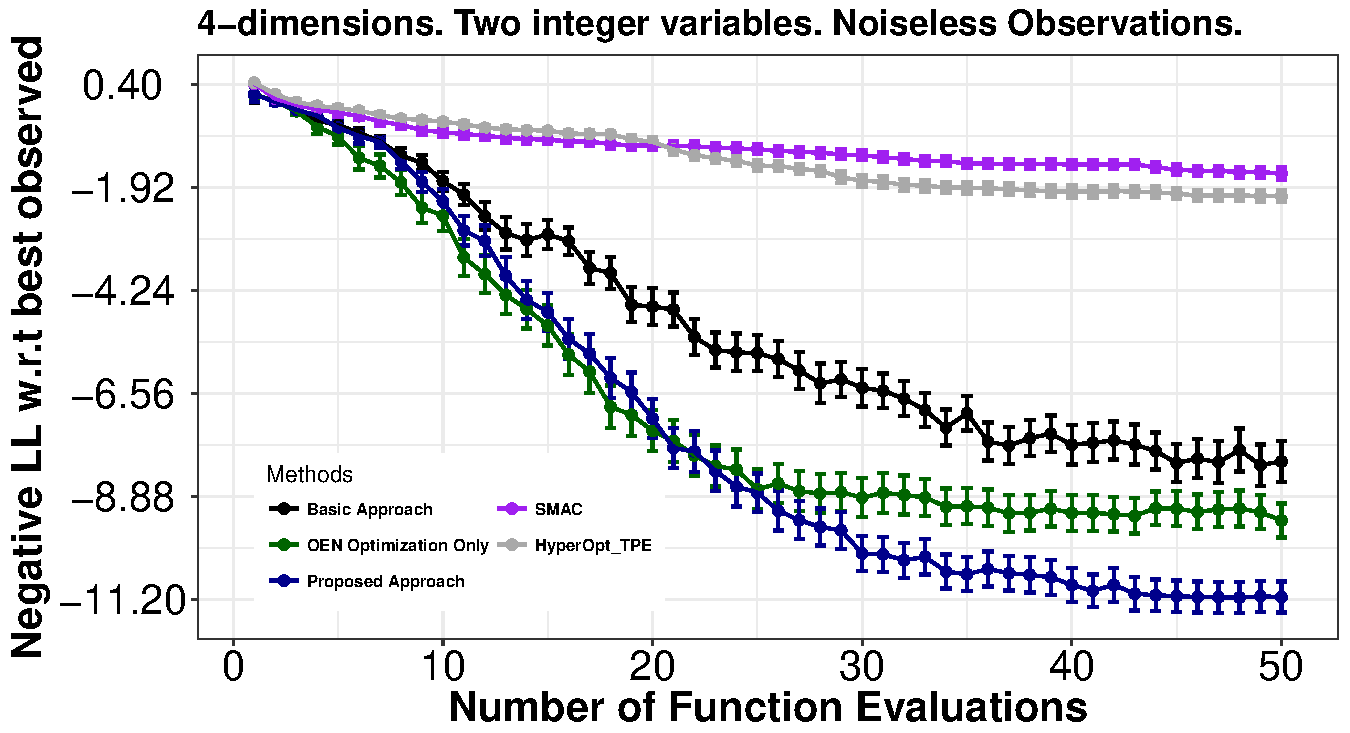
\includegraphics[width=0.475\linewidth]{Figures/integer/synthetic/noiseless/4Dif.pdf} &
        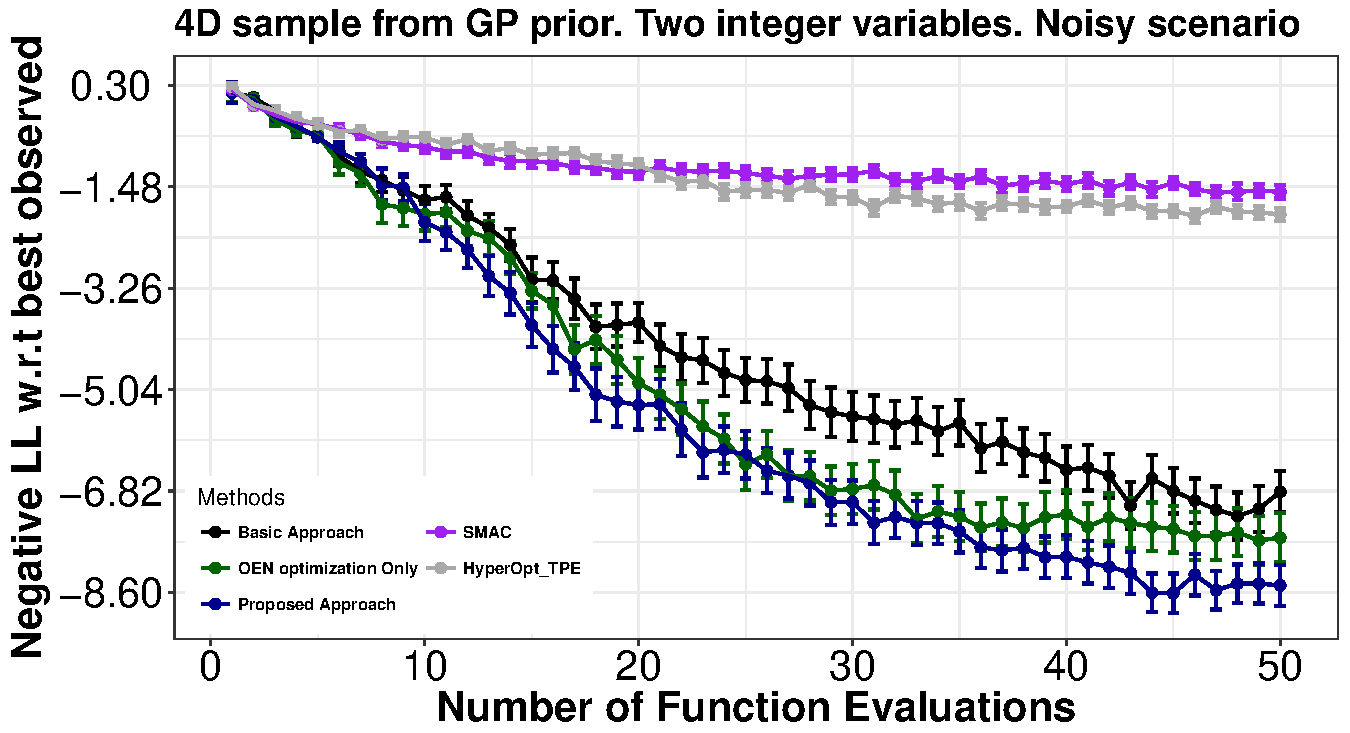
\includegraphics[width=0.475\linewidth]{Figures/integer/synthetic/noisy/4Dinf.pdf} \\
        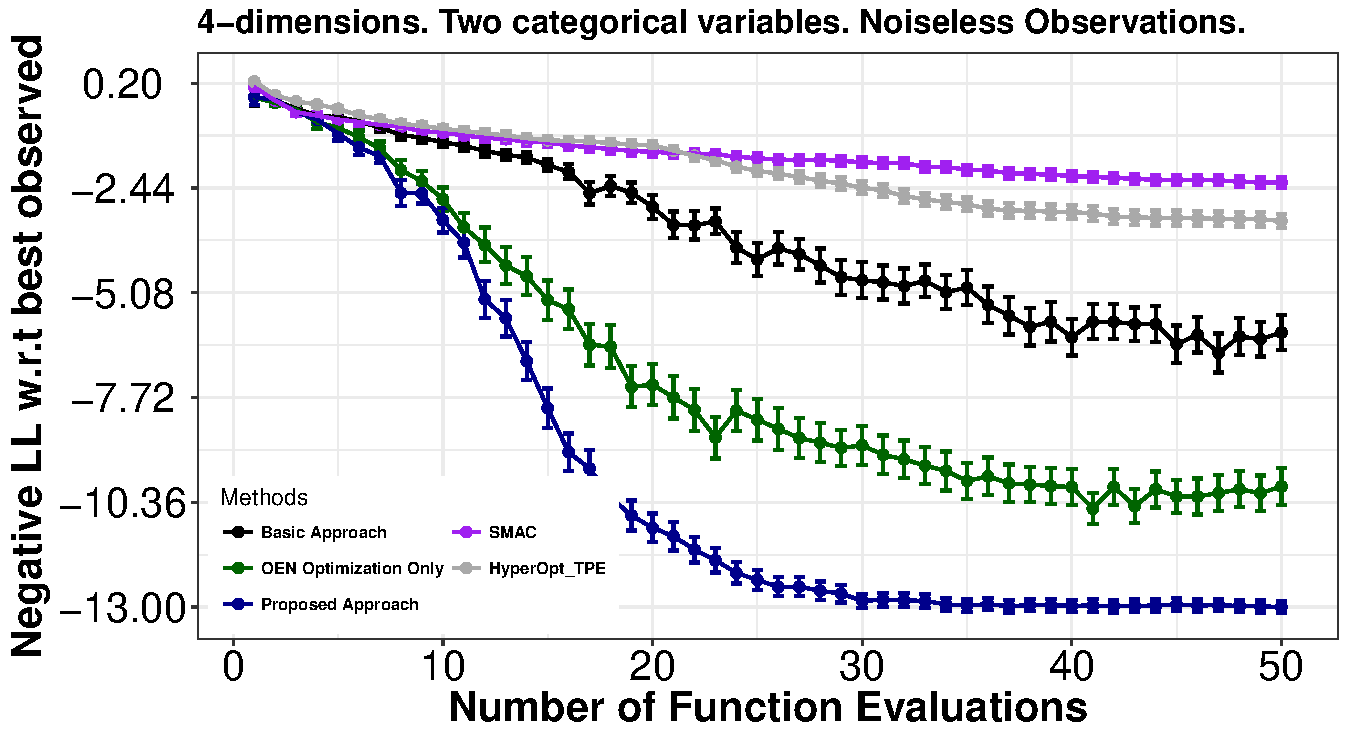
\includegraphics[width=0.475\linewidth]{Figures/integer/synthetic/noiseless/4Dcf.pdf} &
        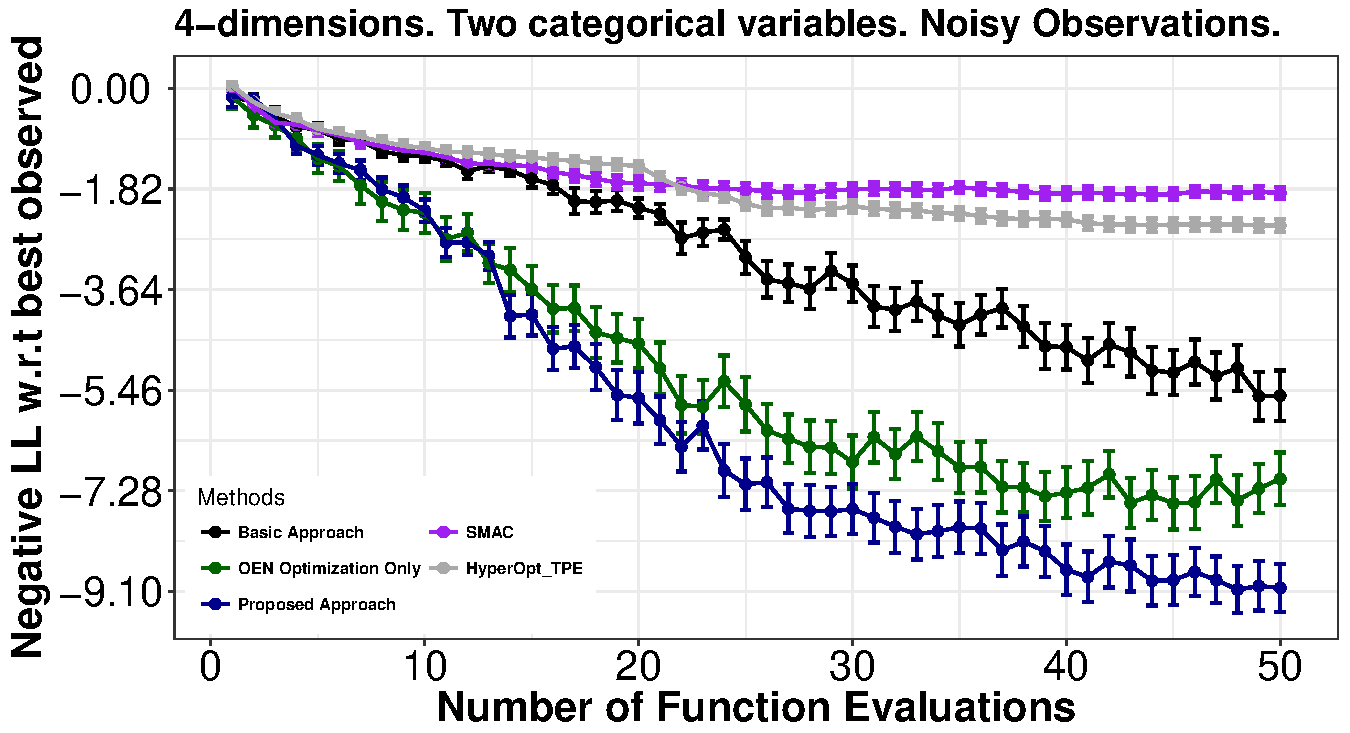
\includegraphics[width=0.475\linewidth]{Figures/integer/synthetic/noisy/4Dcnf.pdf} \\
\end{tabular}
\caption{{\small Average results on the synthetic experiments with 4 dimensions.}}

\label{fig:results_synthetic_4}
\end{figure}

\begin{figure}[htb]
\begin{tabular}{cc}
        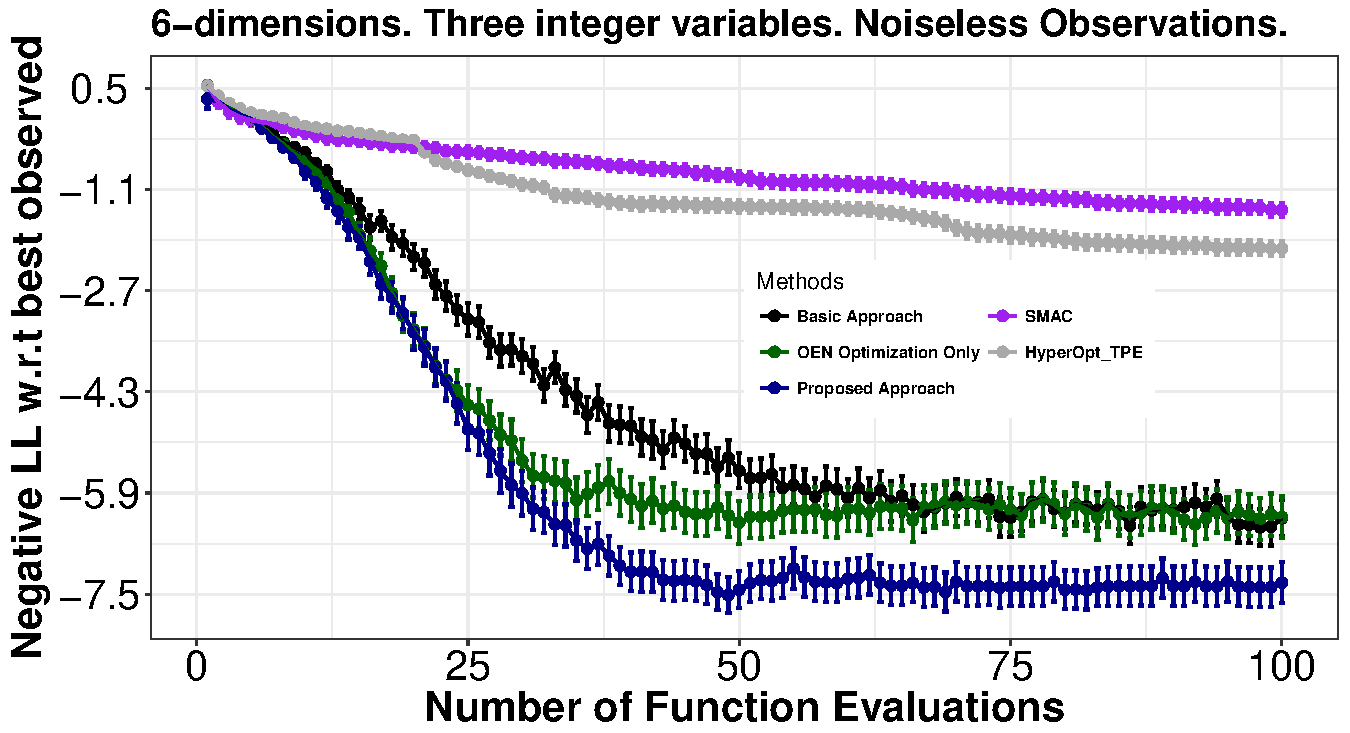
\includegraphics[width=0.475\linewidth]{Figures/integer/synthetic/noiseless/6Dif.pdf} &
        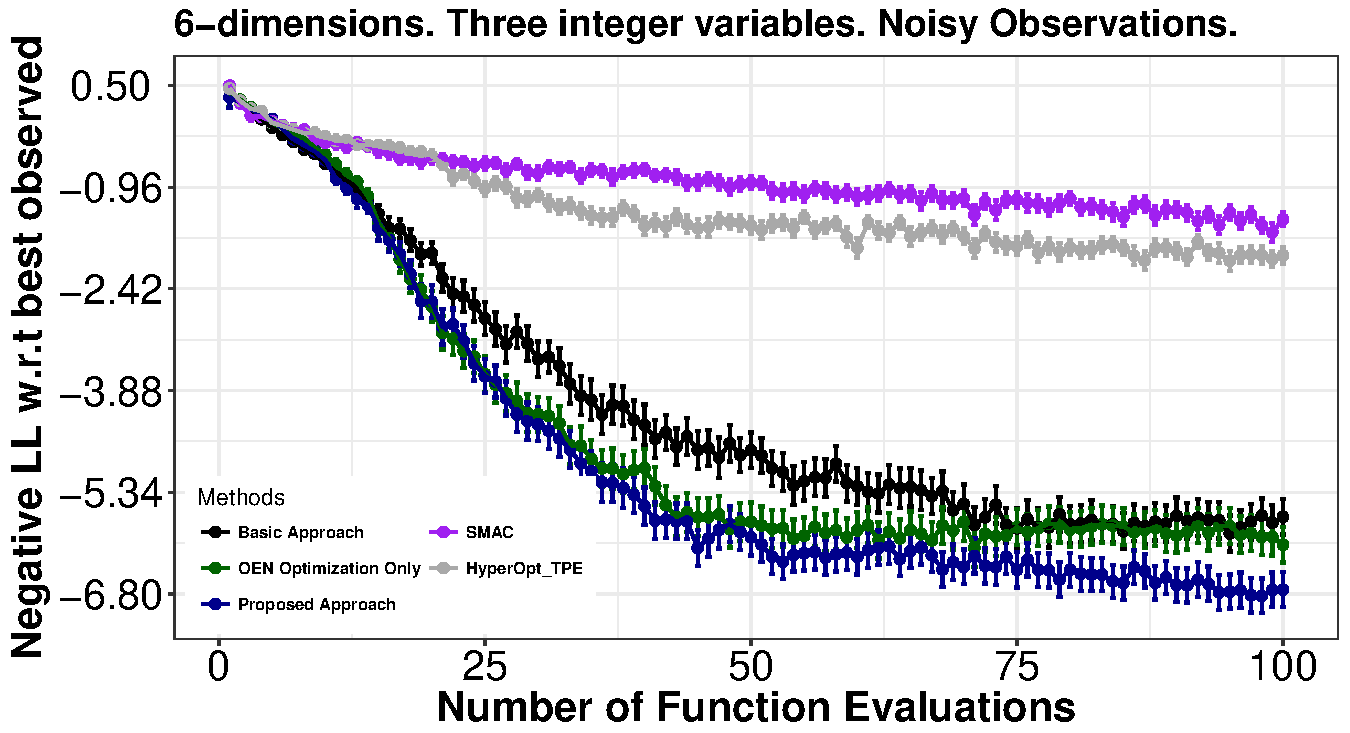
\includegraphics[width=0.475\linewidth]{Figures/integer/synthetic/noisy/6Dinf.pdf} \\
        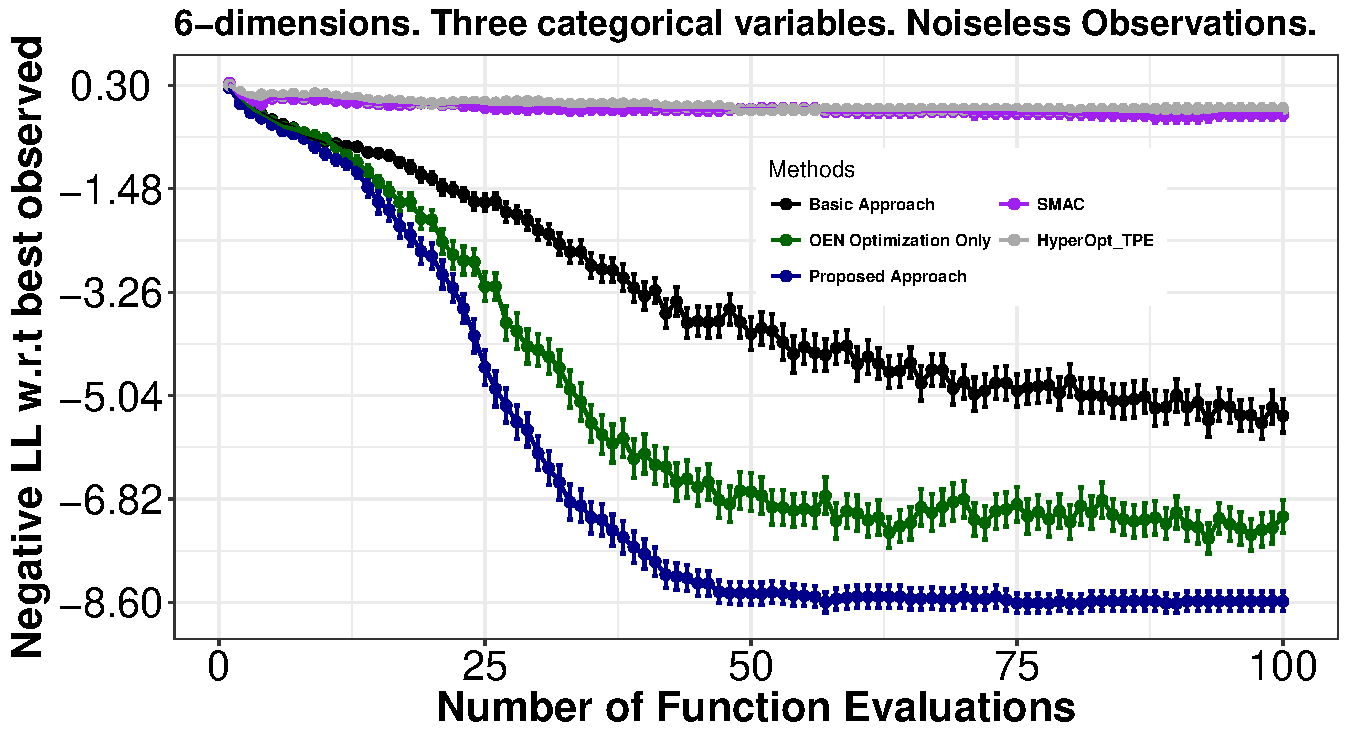
\includegraphics[width=0.475\linewidth]{Figures/integer/synthetic/noiseless/6Dcf.pdf} &
        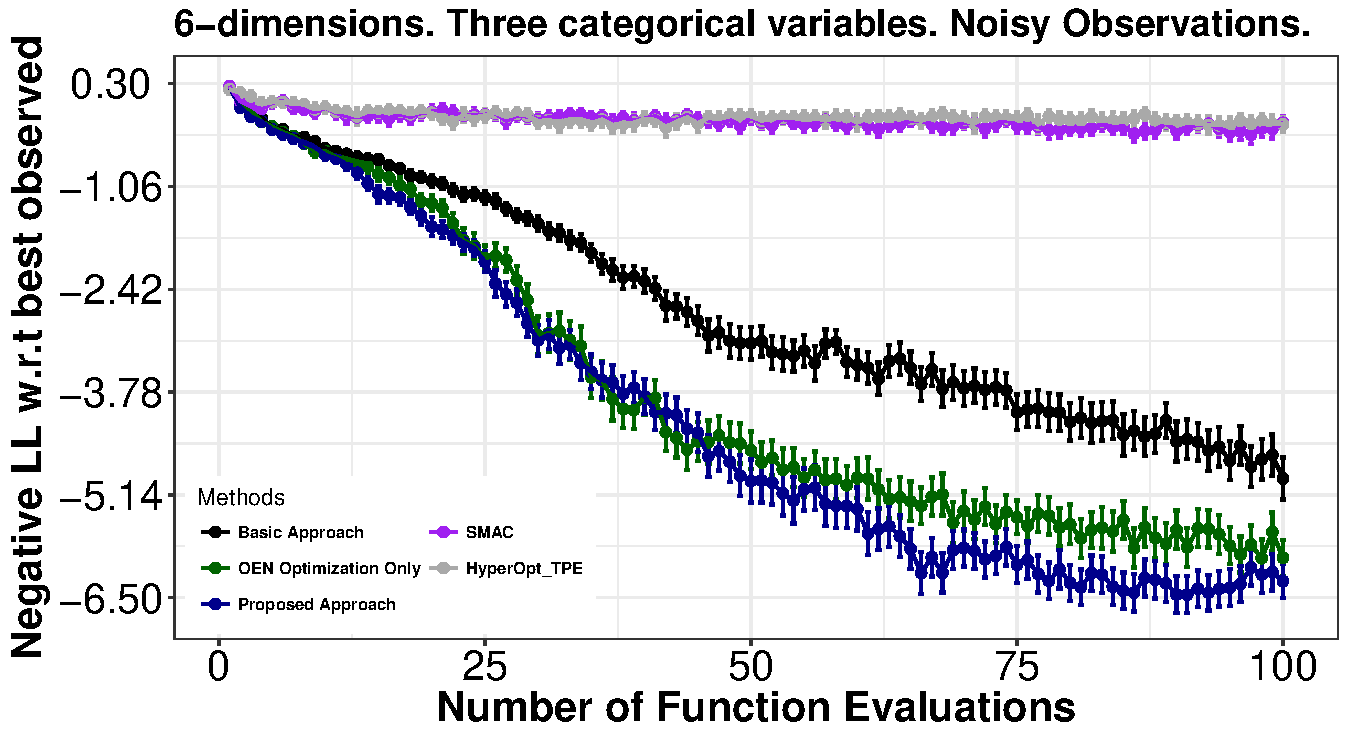
\includegraphics[width=0.475\linewidth]{Figures/integer/synthetic/noisy/6Dcnf.pdf} \\
\end{tabular}
\caption{{\small Average results on the synthetic experiments with 6 dimensions.}}
\label{fig:results_synthetic_6}
\end{figure}

We observe that GP based BO outperforms clearly the non-GP based BO, being the proposed approach better than the basic approach or
the OEN optimization only method. This last method works better than the basic approach, showing that optimizing the acquisition
function with the proposed methodology delivers better results.  In the 6-dimensional scenario the difference of performance between the
basic approach, OEN optimization only and the proposed approach is slightly
higher than in the 4-dimensional scenario. SMAC and TPE also perform worse than the other methods in the 6-dimensional
case. Finally, in the noisy setting, the methods are more equal but the proposed approach works slightly better.
TPE and SMAC also deliver worse results in the noisy setting.

Note that SMAC and TPE do not assume a GP for the underlying model and could be in disadvantage in these experiments.
However, we believe it is still interesting to compare results with them in this setting in which the exact solution
of the optimization problem can be easily obtained and the level of noise can be controlled. In the following section
we carry out experiments in which the actual objectives need not be sampled from a GP, to illustrate the advantages
of the proposed approach in a wider range of problems.

\subsection{Hyper-Parameter Tuning of Machine Learning Algorithms}

We compare all methods on the practical problem of finding the optimal
parameters of a gradient boosting ensemble and a deep neural network on the digits dataset \citep{friedman2001greedy}.
This dataset has 1,797 data instances, 10 class labels and 64 dimensions. It has been
extracted from the python package scikit-learn \citep{scikit-learn}.
Similarly, we also consider finding the optimal hyper-parameters of a deep neural network on
the MNIST dataset \citep{lecun1998mnist}. This dataset has $60,000$ data instances, $768$ dimensions
and $10$ class labels. In this set of experiments, we use Predictive Entropy Search (PES) as
the acquisition function, for both the basic, the proposed approach and the OEN optimization only method.

In the task of finding an optimal ensemble on the digits dataset, the objective that is considered for
optimization is the average test log likelihood of the ensemble. This objective is evaluated using a 10-fold
cross-validation procedure. Note that model bias can be an issue for all methods in this case, since the actual
objective is unknown.  We consider a total of $200$ evaluations of the objective. A summary of the parameters optimized,
their type and their range is displayed on Table \ref{table:1}. These parameters are: The logarithm of the learning rate,
the maximum depth of the generated trees and the minimum number of samples used to split a node in the
tree building process. Importantly, while the first parameter can take real values, the other two can only take integer values.

\begin{table}[htb]
\centering
\caption{Names, types and range of the parameters optimized for the ensemble of trees.}
\begin{tabular}{ l | c | c }
 \hline
 {\bf Name} & {\bf Type} & {\bf Range} \\
 \hline
 Log Learning Rate & Real & $[-10,0]$ \\
 Maximum Tree Depth & Integer & $[1,6]$ \\
 Minimum Number of Samples to Split & Integer & $[2,6]$ \\
 \hline
\end{tabular}
\label{table:1}
\end{table}

In each repetition of the experiment described (there are 100 repetitions) we consider a different 10-fold
cross validation split of the data. The average results obtained are displayed in Figure \ref{fig:results_digits}.
This figure shows the average difference, in absolute value, between the test log-likelihood of the
recommendation made and the best observed test-log likelihood, for that particular split, in a log scale.
We observe that the proposed approach significantly outperforms the basic approach. More precisely, it is able
to find parameter values that lead to a gradient boosting ensemble with a better test log likelihood,
using a smaller number of evaluations of the objective. Furthermore, the proposed approach also performs
better than SMAC, TPE, or the OEN optimization only method.

\begin{figure}[htb]
        \begin{center}
        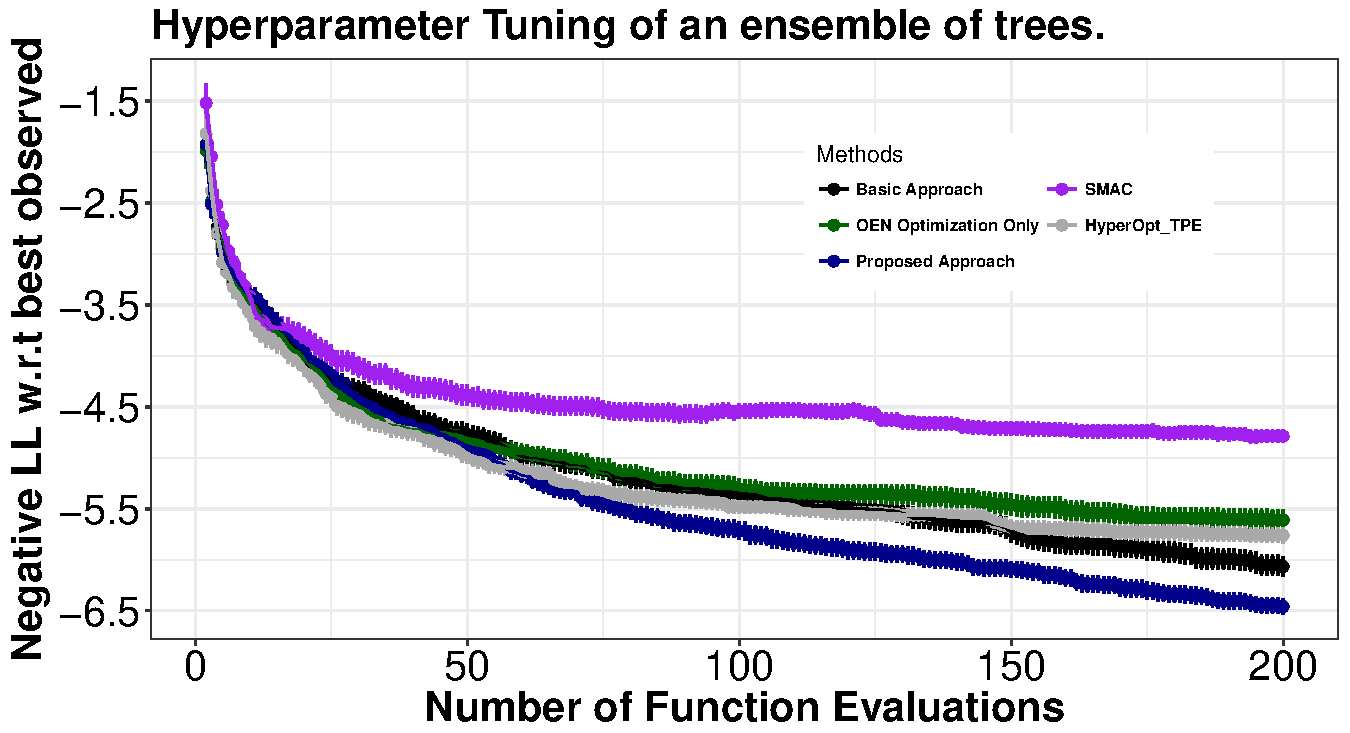
\includegraphics[width=0.7\linewidth]{Figures/integer/real/ensemble_digits_final_ok.pdf} \\
        \end{center}
\caption{{\small Average results on the Digits dataset using Gradient Boosting.}}
\label{fig:results_digits}
\end{figure}

In the task of finding an optimal deep neural network on the digits and MNIST dataset, the objective considered is
the test log-likelihood of the network.  This objective is evaluated using a 10-fold cross-validation procedure in the
digits dataset.  In the MNIST dataset a validation set of $10,000$ instances, extracted from the training set is used.
We consider $125$ and $150$ evaluations of the objective for the digits and the MNIST dataset, respectively.
A summary of the parameters optimized, their type and their range is displayed on Table \ref{table:2}. These parameters
are: The logarithm of the learning rate, the activation function and the number of hidden
layers. The first parameter can take values in the real line. The second and third
parameters are categorical and integer-valued. The number of units in each layer, is set
equal to $75$.

\begin{table}[htb]
\centering
\caption{Name, type and range of the deep neural network parameters optimized.}
\begin{tabular}{ c | c | c }
 \hline
 {\bf Name} & {\bf Type} & {\bf Range} \\
 \hline
 Log Learning Rate & Real & $[-10,0]$ \\
 Activation Function & Categorical & Linear, Sigmoid, Tanh or ReLU \\
 Number of hidden layers & Integer & $[1,3]$ \\
 \hline
\end{tabular}
\label{table:2}
\end{table}

The average results obtained in the two classification problems are displayed in Figure \ref{fig:results_deep}.
The figure shows the average difference, in absolute value, between the test log-likelihood
of the recommendation made and the best observed test-log likelihood, in a log scale.
Again, the proposed approach significantly outperforms the basic approach. More precisely, it is able
to find parameter values that lead to a deep neural network with a better test log likelihood
on the left-out dataset, using a smaller number of evaluations of the objective. The proposed approach
also outperforms SMAC. However, on the MNIST dataset, TPE is only slightly worse than the proposed approach at
the end and it outperforms the basic approach. We believe that the better results of TPE obtained in this
problem can be a consequence of model bias in the GP that is used to fit the objective in the
proposed approach. In both problems, the proposed approach outperforms the OEN optimization only method and the basic approach.

\begin{figure}[htb]
        \begin{center}
        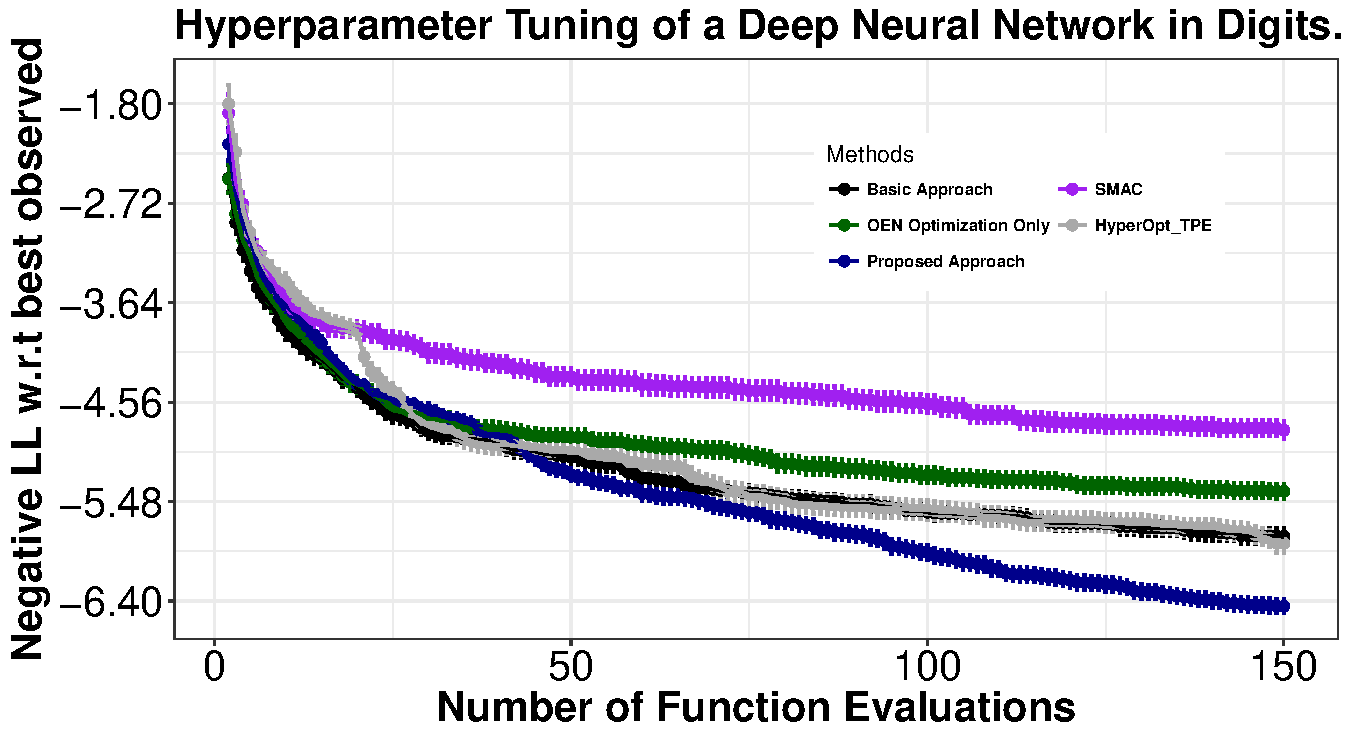
\includegraphics[width=0.7\linewidth]{Figures/integer/real/rrnn_digits_final_ok.pdf} \\
        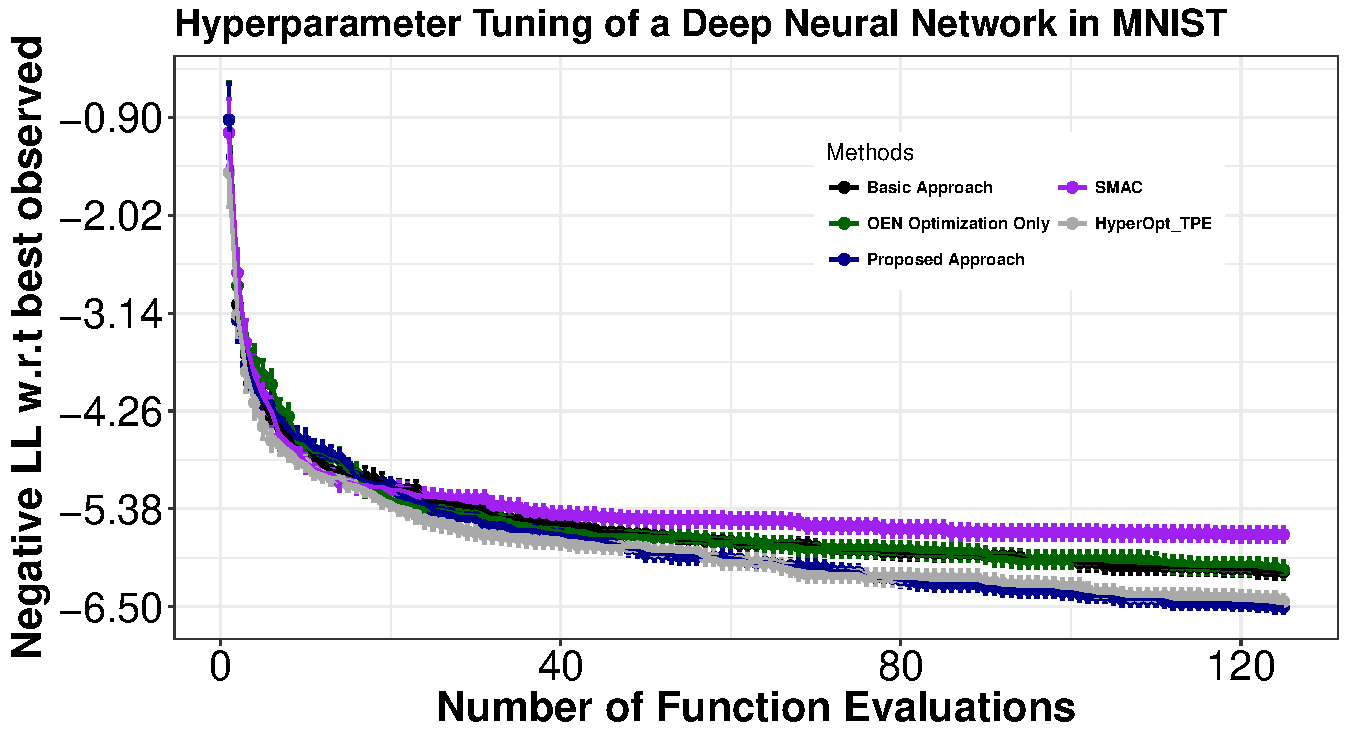
\includegraphics[width=0.7\linewidth]{Figures/integer/real/rrnn_final_ok.pdf} \\
        \end{center}
\caption{{\small Average results on the Digits and MNIST dataset using deep neural networks.}}
\label{fig:results_deep}
\end{figure}

\subsection{Experimenting with the Combinatorial-Valued Variables Transformation}
The full representation of a combinatorial-valued variable make the execution of experiments with it infeasible due to the high number of dimensions required by a GP to model the combinatorial-valued variable. The computers that run the experiments suffer from system errors due to not enough memory to model all the dimensions required by the full transformation. For example, in the case of having $8$ dimensions in the combinatorial-valued variable, the full transformation required $256$ dimensions, making it infeasible in practice.

\begin{figure}[htb]
\begin{tabular}{cc}
        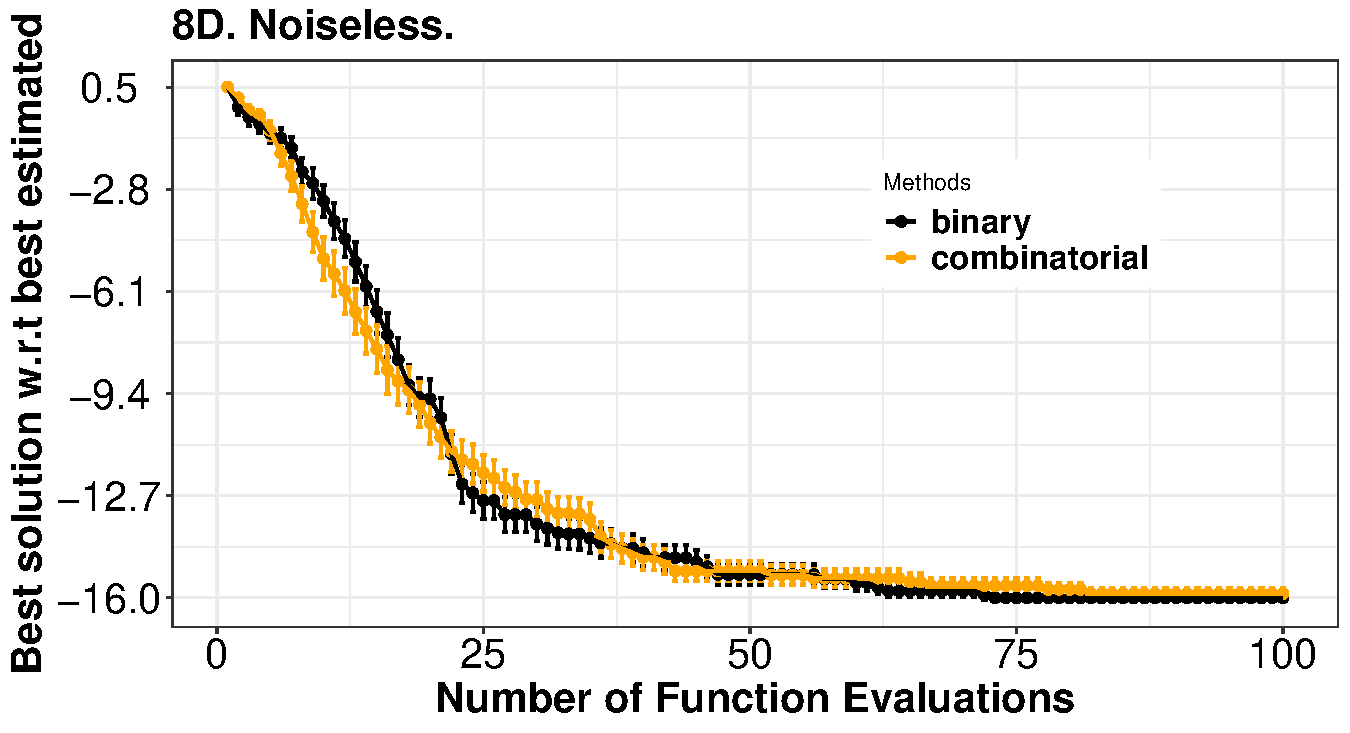
\includegraphics[width=0.475\linewidth]{Figures/combinatorial/8V.pdf} &
        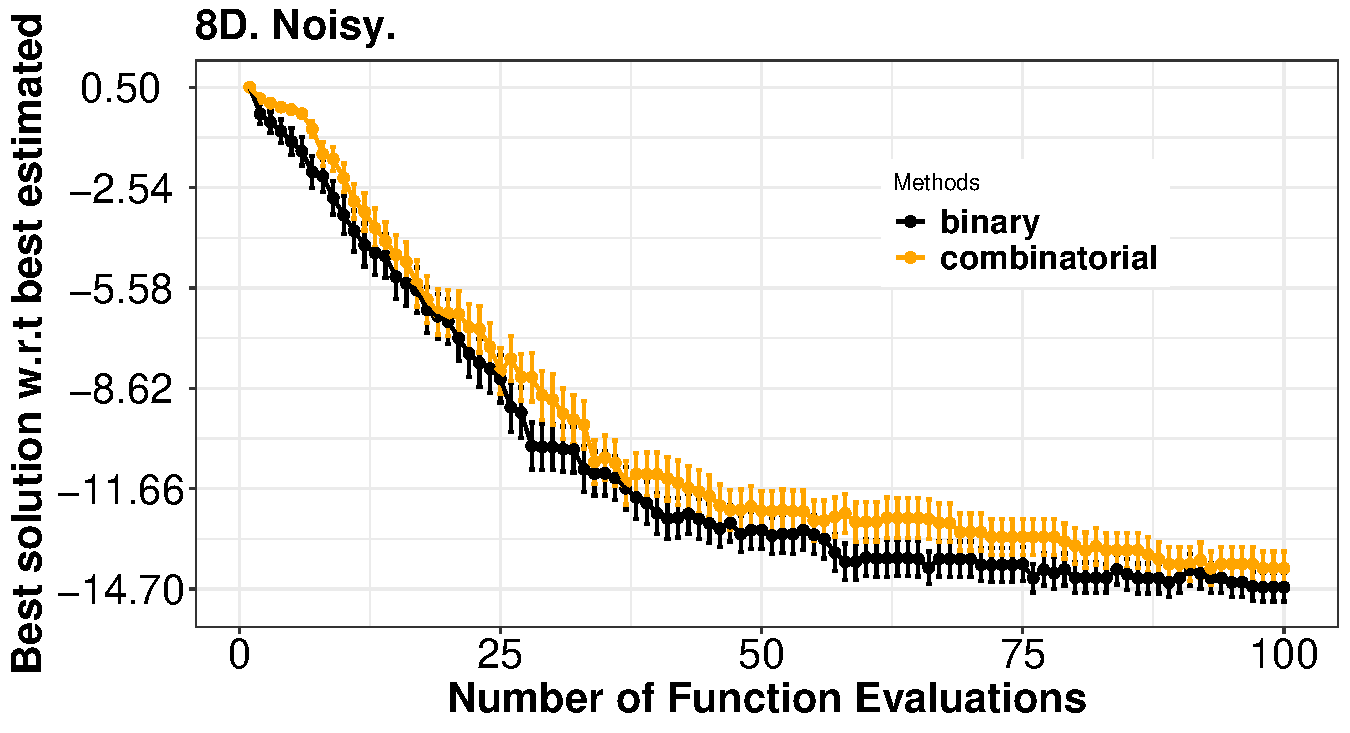
\includegraphics[width=0.475\linewidth]{Figures/combinatorial/8V_noisy.pdf} \\
        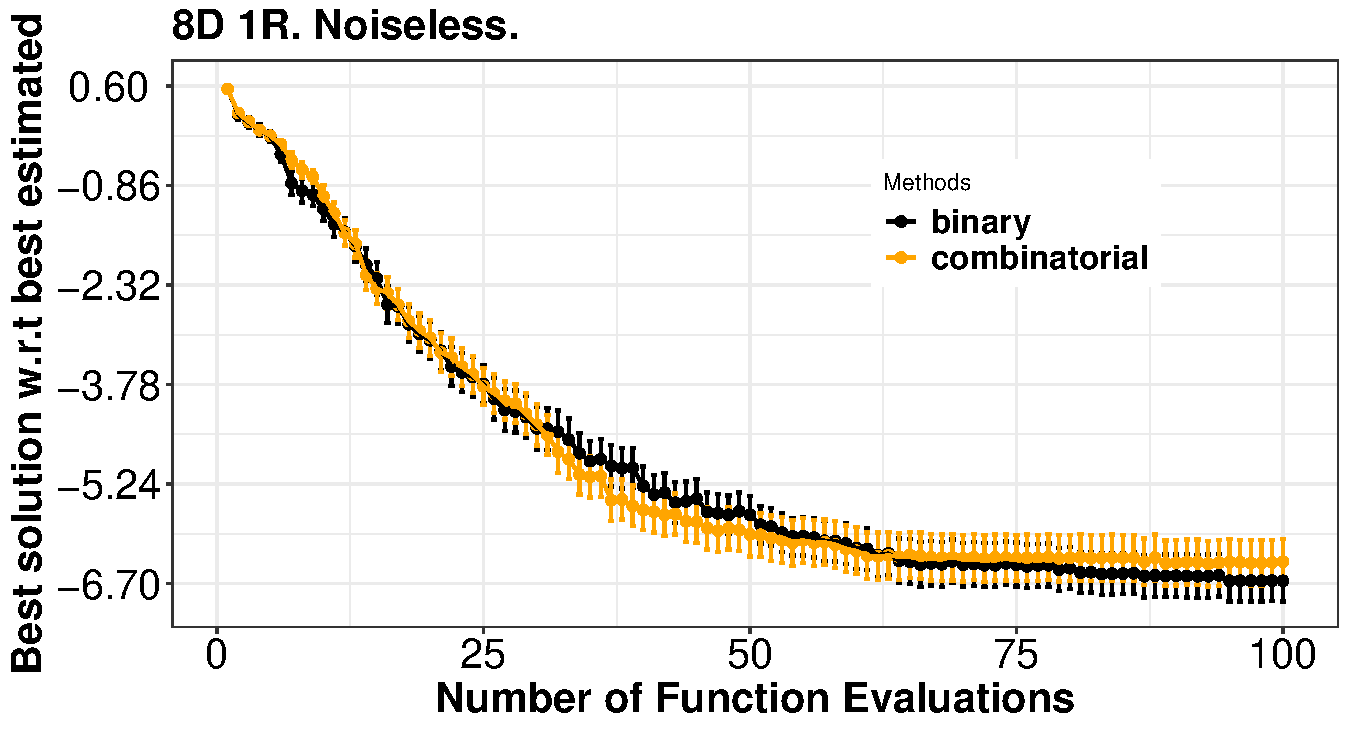
\includegraphics[width=0.475\linewidth]{Figures/combinatorial/8V1R.pdf} &
        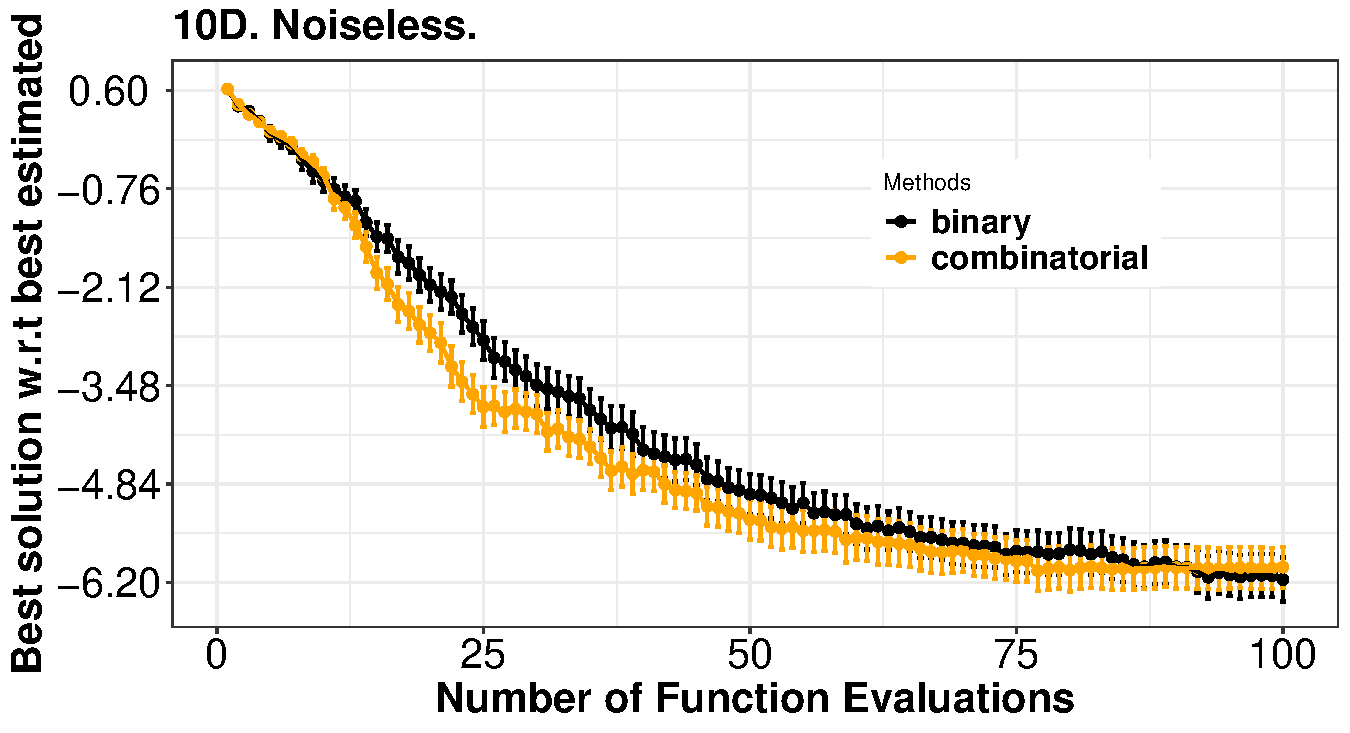
\includegraphics[width=0.475\linewidth]{Figures/combinatorial/10V.pdf} \\
\end{tabular}
\caption{{\small Average results on the synthetic experiments.}}
\label{fig:results_synthetic_combinatorial}
\end{figure}
\section{Conclusions}
Results of the combinatorial transformation do not considerably improve the performance the ones of the binary transformation of the variable. Although we gain some performance, possibly because of the GP requiring less dimensions to model the problem, is not very significant. Real experiments may provide different results. Although, the combinatorial-valued transformation required a lower number of dimensions than the binary transformation and, hence, consumed less memory, which it is a significant advantage with respect to the binary transformation.
